\documentclass[a4paper,10pt]{scrreprt}
\usepackage[utf8]{inputenc}
\usepackage{graphicx}
\usepackage{hyperref}
% hide link borders
\hypersetup{
    colorlinks=false,
    pdfborder={0 0 0},
}
\usepackage{color}
\usepackage{amsmath}
%\usepackage{float}
\usepackage{listings}
\usepackage{appendix}
\usepackage[section]{placeins}
\usepackage{wrapfig}
\usepackage{pdfcomment}
\usepackage{parskip}
\usepackage[toc,xindy]{glossaries}
%\usepackage[nottoc,numbib]{tocbibind}
\usepackage{changepage}

\newacronym{DNA}{DNA}{deoxyribonucleic acid}
\newacronym{RNA}{RNA}{ribonucleic acid}
\newacronym{BSA}{BSA}{biological sequence analysis}
\newacronym{SciWMS}{SciWMS}{scientific workflow management system}
\newacronym{XML}{XML}{Extensible Markup Language}
\newacronym{VPL}{VPL}{visual programming language}
\newglossaryentry{bsanalysis}{
name={biological sequence analysis},
description={is the process of inferring biological knowledge from the sequence of biological molecules such as \gls{DNA} and \gls{RNA}. Broadly speaking, knowledge is either gleaned ab initio, that is by applying models to the sequence itself, or by comparing new sequence to known sequence, using a \gls{homology} search}
}
\newglossaryentry{homology}{
name={sequence homology},
description={is a feature of sequences that share common evolutionary ancestry. Typically such sequences will share a degree of sequence similarity. In other words, sequences of \glspl{gene} that perform similar functions will ``look'' somewhat similar, and this similarity can be searched for using tools such as \gls{BLAST}},
plural={sequence homologies}
}
\newglossaryentry{BLAST}{
name={BLAST},
description={is the Basic Local Alignment Search Tool \cite{altschul_gapped_1997}, a program used by biologists to execute \gls{homology} searches. Using BLAST one or more query sequences can be search against a database of \glspl{nucleicacid} or \glspl{protein} to find sequences to which it is similar}
}
\newglossaryentry{gene}{
name=gene,
description={is a molecular unit of genetic information. All living organisms use gene to store the genetic information that both provides a recipe for the construction of protein and allows for inheritance of traits from one generation to the next},
plural=genes,
}
\newglossaryentry{aminoacid}{
name={amino acid},
description={is one of a family of biological molecules used in the construction of \glspl{protein}},
plural={amino acids}
}
\newglossaryentry{protein}{
name={protein},
description={is a macromolecule that performs a biological function in a living organism. Proteins are constructed out of \glspl{aminoacid} and a major function of \gls{DNA} is to store the \glspl{gene} that describe the sequences of \glspl{aminoacid} out of which proteins are constructed},
plural={proteins}
}
\newglossaryentry{nucleicacid}{
name={nucleic acid},
description={is a biological molecule. \gls{DNA} is a nucleic acid that stores the genetic information of a cell. \gls{RNA} is another nucleic acid that is involved, amongst other things, in the transport of genetic information and the construction of protein},
plural={nucleic acids}
}
\newglossaryentry{base}{
name={base},
description={is an informal term for a nucleobase, the molecular units out of which \glspl{nucleicacid} are constructed. In \gls{DNA} there are four types of base: adenine, guanine, thymine and cytosine. These are typically represented by the letters A, G, T and C. In \gls{RNA} thymine is replaced by urasil, denoted by the letter U},
plural={bases}
}
\newglossaryentry{sequencing}{
name={sequencing},
description={refers to the process of determining the order of the nucleotide \glspl{base} in a \gls{nucleicacid}},
}
\newglossaryentry{workflow}{
name=workflow,
description={is a description of the sequences of procedures necessary to undertake a particular process. In this regard workflows are similar to laboratory protocols in that they describe a reproducible set of steps that need to be undertaken to perform a scientific analysis},
plural=workflows
}
\newglossaryentry{SciWMSystem}{
name={scientific workflow management system},
description={is a application or set of applications that allows users to composer and execute scientific \glspl{workflow} using a given set of design primitives},
plural={scientific workflow management systems},
}
\newglossaryentry{opensource}{
name={open source software},
description={is software developed according to a philosophy that promotes free redistribution and access to the design and implementation details of the software product. This means that source code and sometimes binaries for the software are available for users to freely redistribute and alter}
}
\newglossaryentry{XMLang}{
name={Extensible Markup Language},
description={is a markup language that defines a set of rules for encoding documents in such as way as to be readable by both machines and humans}
}
\newglossaryentry{visualpl}{
name={visual programming language},
description={is a kind of programming language where the elements of computation are expressed using graphical diagrams. As with textual programming languages, some form of interpreter or compiler takes the user created program diagram as input and converts it into instructions that can be executed on a computer},
plural={visual programming languages}
}
\newglossaryentry{controlflow}{
name={control flow},
description={refers to the order in which individual elements of computation (statements or tasks) are executed. Control flow operators (such as iteration and choice) express the paths that execution might proceed through a program, and the conditions attached to those paths. For example, the ``if'' statement available in most programming languages directs execution along a particular path only if a certain condition is true. Contrast with \gls{dataflow}}
}
\newglossaryentry{dataflow}{
name={dataflow},
description={refers to the dependencies that exist between elements of data in a program or computational system. For example, the average length of a set of strings depends on the set of strings. Dataflow does not specify in what order computation needs to proceed, as opposed to \gls{controlflow}}
}
%\newglossaryentry{homology}{
%name={homology},
%description={refers to similarity between nucleotide or amino acid sequences that is an indicator of shared evolutionary ancestory. It may also be indicative of shared
%function, that is two similar nucleotide or amino acid sequences maybe both go on to create biological molecules that ``work'' the same way.}
%}
%\newglossaryentry{BLAST}{
%name={BLAST},
%description={the Basic Local Alignment Search Tool, is a tool used in bioinformatics for doing homology, that is sequence similarity, searches. Using BLAST involves a
%pre-processing step where the database of sequences to be searched is formatted in BLAST database format. Once this database is created, it can be searched 
%rapidly to find matches (known as hits) for a given query sequence.}
%}
\newglossaryentry{ortholog}{
name={ortholog},
description={a gene that is related to another gene by a shared history. Two genes, in two different species or two different forms of the same species, are orthologs if
they evolved from the same gene at some point in the organism's history. The difference between two orthologous genes can be small, for example one letter of DNA might
be an `A' in the one and a `G' in the other, or it might be larger, but in general a sequence similarity (aka. homology) search will show that the genes are similar.},
plural={orthologs}
}
\makeglossary
\glsaddall

%opening
\title{The Computer Scientist's Guide to Galaxy}
\subtitle{An evaluation of the Galaxy workflow system's ability to address the challenges of bioinformatics}
\author{Peter van Heusden\\
student number: 45764980}

\begin{document}



\bibliographystyle{alpha}

\maketitle

\begin{abstract}
My abstract
\end{abstract}

\tableofcontents

\listoffigures

\chapter{Introduction and Motivation}


Bioinformatics is the discipline of solving problems in biology and medicine using computational resources (databases, analysis programs, etc). Within this field \gls{BSA}\footnote{While the objects of study in bioinformatics range beyond biological sequences, this research focuses on \gls{BSA} since it makes up such a large part of day to day bioinformatics workloads. In Stevens et al \cite{stevens_classification_2001}'s (albeit dated) survey of tasks in bioinformatics, 254 out of 315 activities undertaken by the respondents were clearly \gls{BSA}.} covers those analyses that ``infer biological information from sequence alone'' \cite[p.~1]{durbin_biological_1998}. As far back as 1998, Richard Durbin and his co-authors recognised that the development of widely available and accessible genome sequencing would lead to a great acceleration in the accumulation of biological knowledge. Data from the US National Human Genome Research Institute shows that between 2000 and 2012 the cost of \gls{sequencing} \gls{DNA} has decreased at an exponential rate \cite{national_human_genome_research_institute_dna_2012}, and this cost decline has seen a concomitant increase in the amount of genomic sequence data from which biological knowledge can be inferred \cite{cochrane_international_2010}. \begin{wrapfigure}{r}{0.6\textwidth}
  \vspace{-10pt}
  \centering
    \includegraphics[width=0.58\textwidth]{images/seqgrowth.png}
  \vspace{-10pt}
  \caption{Growth of sequence content of public databases, from \cite{cochrane_international_2010}}
  \vspace{-10pt}
\end{wrapfigure}Raw DNA sequence data does, however, equate to biological knowledge. This data needs to be analysed, a process that combines human skill (the ability to translate biological questions into computational procedures) with computational infrastructure. With the cost of computing infrastructure steadily dropping (although not at a pace as fast as the cost of DNA sequencing drops), the human element in analysing biological data will tend to dominate the cost of producing knowledge in bioinformatics to an ever greater degree, unless innovations in the work process of \gls{BSA} keep pace with the explosion in available data (and the implosion of sequencing costs).

In addition to the problem of cost structure in bioinformatics, some experts in the field suggest that there are simply not enough bioinformaticists to keep up with the data deluge. Mabey et al \cite{mabey_report_2005} suggest that ``the rate of growth of [bioinformatics], and its cross-disciplinary nature, has created a problem: while there are many trained biologists and computer scientists, there are few computer-literate biologists or biology-literate computer scientists.'' To put this shortage in perspective, at the South African National Bioinformatics Institute (SANBI), South Africa's largest bioinformatics centre, student enrollment grew from 8 in 2001 to 31 in 2008, an approximately fourfold increase \cite{south_african_national_bioinformatics_institute_south_2010}. During the same period, the amount of data in public sequence databases grew approximately 100-fold.  In addition, the growth in both the amount of data that requires analysis, and the computational power used to analyse such data, 
inevitably leads to requirements for more complex data analyses. What might once have been sequential analysis run by hand on a single server, with results stored in a researcher's folder on disk might now become parallel analysis run on a cluster or grid of computers, with results stored in some form of database. This requirement for increased sophistication in the computational side of \gls{BSA} puts further pressure on bioinformaticists, many of whom have a background in life sciences and limited computer science training. \footnote{A survey I conducted of 16 randomly selected postgraduate students at SANBI revealed that 11 (69\%) of them had been life sciences students as undergrads, 3 (19\%) of them came from mathematical and statistical science backgrounds, and only 2 (12\%) had been exposed to computer science prior to adopting bioinformatics as a field of study.} The sudden on reliance on computation for \gls{BSA} has resulted in what some have called a \emph{informatics crisis} for researchers in 
the field \cite{goecks_galaxy:_2010}, and this in turn has spurred a search for ways to make computing more accessible for researchers.

\Glspl{SciWMSystem} have been proposed as a solution to make computing resources accessible to research scientists in their question to analyse ever larger datasets. \cite{deelman_workflows_2009} A \gls{SciWMS} is a software tool that allows for the orchestration of the \glspl{workflow} that describe the procedures of scientific data analysis. These procedures typically involve moving data to or from computing resources (i.e. staging), launching and managing computation, and managing the output of computation, either storing it in a data store for future reference, or passing it on to the next stage in analysis. This research will focus on one particular \gls{SciWMS}: Galaxy.

%and their While Abouelhoda et al suggest that \glspl{SciWMS} ``provide an easy-to-use metaphor that can be used for both designing and executing bioinformatics application''. \cite{abouelhoda_meta-workflows:_2010}

Since 2009, the ``Pipelines'' collaboration between SANBI \cite{pipelines_working_group_bio-analysis_2011} and researchers at the University of Cape Town has been investigating tools that can be used to rapidly assemble \glspl{workflow} for \gls{BSA}.\footnote{The name of the group derives from the term ``sequence analysis pipeline'', where pipeline is synonymous with workflow. More information about the ``Pipelines'' group can be found at \href{https://pipelines.sanbi.ac.za}{the Pipelines website}.} In the context of this research the Galaxy platform \cite{giardine_galaxy:_2005} was chosen as a platform for rapid development of \gls{BSA} \glspl{workflow}. Experience with this framework and with the broader problem of enabling non-programmers\footnote{In this context non-programmers refers to users that are neither experts in application programming languages such as Java and C++, nor are they experts in using scripting languages such as Perl and Python} to perform \gls{BSA} inspired the topic of this 
research. The objective of this research is to evaluate Galaxy as a \gls{SciWMSystem} for \gls{bsanalysis}.

This evaluation will proceed in two parts. In chapter \ref{sec:intro_swms} \gls{SciWMS} will be examined in detail, to understand how they might make computation accessible to non-programmers and how their expressive power and features relate to tasks in bioinformatics. Building on the existing literature and case studies of real world bioinformatics problem solving, a set of criteria for evaluating \glspl{SciWMS} will be introduced. Then, in chapter \ref{sec:galaxy_swms} Galaxy will be introduced and evaluated in terms of the criteria introduced in chapter \ref{sec:intro_swms}. Features provided by and absent in Galaxy will be highlighted. Finally, conclusions will be drawn about Galaxy's strengths and weaknesses, with reference to the central problem of making the authoring and execution of analyses more efficient and accessible. Directions for possible future work will be also be highlighted.

%the Galaxy platform will be introduced, and its relevant component described (Section %\ref{sec:galaxyexplained}). Then a theoretical model of tasks in bioinformatics will be presented (Section %\ref{sec:tasksinbioinformatics}) and this theoretical model will be fleshed out with three case studies of %real world \gls{BSA} \glspl{workflow}, These case studies will consider how these \glspl{workflow} can be %implemented using Galaxy, and also how they relate the model provided in Section %\ref{sec:tasksinbioinformatics}. Thirdly, a framework for evaluating \gls{workflow} systems will be %introduced and the Galaxy workflow system will be evaluated using this framework. Finally conclusions will %be drawn and future directions of research will be discussed.

%Galaxy is a workflow system used in the field of bioinformatics, and has been proposed as a solution to the ``informatics crisis'' facing genome
%biology. \cite{goecks_galaxy:_2010} The object of my research is to evaluate to what extent Galaxy is, in fact, an appropriate tool for bioinformatics, with a particular focus on \gls{BSA}. In the course of doing this evaluation, I will situate Galaxy within the larger field of scientific workflow systems, in order to illuminate what features are particular to the Galaxy environment, in order to assess to what extent, and how, scientific workflow systems can contribute to the task of producing biological knowledge from the current wealth of genomic data.
 
\chapter{Introduction to scientific workflow systems}
\label{sec:intro_swms}

The notion of a \gls{workflow} originated in the study of business processes and the 1995 Workflow Management Coalition's reference model describes a \gls{workflow} in terms of ``procedures where documents, information or tasks are passed between participants according to a defined set of rules to achieve, or contribute to, an overall business goal'' \cite{hollingsworth_workflow_1995}. According to Abbott et al, the need for workflow management in business was driven by the challenges of coordinating work taking place on large numbers of desktop computers interconnected in a network \cite{abbott_experiences_1994}. \Glspl{workflow} in business are realised using a workflow management system that defines, manages and executes workflows on computational resources \cite{yu_taxonomy_2005}. 

While the concept of \glspl{workflow} was first applied to business processes, there are now many \glspl{SciWMS}. These aim to model and enact \glspl{workflow} that ``[support] large-scale, complex, yet fault-tolerant and maintainable scientific processes'' \cite{yildiz_towards_2009}. Castro et al describe \glspl{workflow} as analogous to laboratory protocols, that is allowing scientists to provide ``rich descriptions of their experiments (materials and methods) so they can be easily replicated'' \cite{castro_workflows_2005}. Yildiz et al \cite{yildiz_business_2009} note that scientific workflows are distinguished from business workflows by being``dataflow oriented'': whereas business workflows focus on the set of activities that take place to enact a business process, scientific workflows focus on the flow of data between tasks in an analytical process.

If \glspl{SciWMS} in general, and Galaxy in particular, are to help solve the \emph{informatics crisis} in bioinformatics, two questions need to be answered: Firstly, can \glspl{SciWMS} make computation more accessible for non-programmers? Abouelhoda suggest that \glspl{SciWMS} provide an ``easy-to-use metaphor that can be used for designing and executing bioinformatics applications''. Empirical research on \glspl{VPL}\footnote{Most \glspl{SciWMS} use some form of graph-based \gls{VPL} to compose \glspl{workflow} \cite{yu_taxonomy_2005}.} done by Blackwell et al suggests that metaphor, on its own, is not a significant factor in guiding people's understanding of how to compose or understand program logic \cite{blackwell_does_1999}. Instead they suggest \cite{blackwell_cognitive_2001} that Green et al's model of thirteen cognitive dimensions of programming environments should be used to judge the accessibility of a \gls{VPL}. 

In addition Blackwell et al point to the role that a large library of reuseable components play in the expressive power of programming environments\footnote{Both the Galaxy (\cite{giardine_galaxy:_2005} and \cite{nekrutenko_introduction_2011}) and Taverna \cite{hull_taverna:_2006} developers highlight the range of pre-existing components available for use in their \glspl{SciWMS}} and also the importance of choosing a paradigm that ``maps'' to the user's understanding of their problem domain. McPhillips et al  suggest that since scientific computation involves successive steps of analysis of collections of data, the dataflow paradigm\footnote{The dataflow paradigm is embodied by a set of programming languages and environments where computation is expressed in terms of the flow of data between computing steps. See for example \cite{gostelow_view_1979} and \cite{lee_dataflow_1995}. This paradigm is contrasted with ``control flow'', where computation is expressed in terms of the flow of control in a program. Lee 
et al \cite{lee_dataflow_1995} suggest that whereas in the control flow paradigm programming is imperative, that is, the job of the user is to tell the computer what to do at each step, the dataflow paradigm emphasises declarative design, where the user specifies inputs and outputs but does not necessarily specify the detail of how computation is executed.} is appropriate for \glspl{SciWMS}. They propose eight desirable characteristics that assist in the adoption of \gls{SciWMS} by scientist who are not programmers. Green et al and McPhillips et al's schemas are introduced in section \ref{sec:eval_swms_usability} and they are used to evaluate Galaxy in section \ref{sec:galaxy_swms_useability}.

There is a second perspective from which \glspl{SciWMS} and Galaxy must be considered if they are to be useful for \gls{BSA}. How can we know if these systems can efficiently express the necessary computational constructs necessary to undertake \gls{BSA}? Stevens et al \cite{stevens_classification_2001} and Castro et al \cite{castro_workflows_2005} have provided a theoretical model of tasks encountered in bioinformatics. This model is discussed in Section \ref{sec:bioinformatics_tasks}. In order to validate this model and provide more practical understanding of the tasks undertaken in \gls{BSA}, three cases studies are presented in section \ref{sec:case_studies} that present real world examples of how problems in \gls{BSA} have been solved. Having established an understanding of what is involved in \gls{BSA}, a framework for evaluating \glspl{SciWMS} will be presented. Van der Aalst et al and have identified a set of workflow patterns, where patterns are ``abstraction[s] from a concrete form which [keep] 
recurring in specific nonarbitrary contexts'' \cite{van_der_aalst_workflow_2003}. Yildiz et al \cite{yildiz_towards_2009} have applied van der Aalst et al's insights to the study of \gls{SciWMS}. These patterns will be considered in the context of the model of computation in \gls{BSA} in section \ref{sec:workflow_patterns}, and the extent to which Galaxy supports these patterns will be discussed in section \ref{sec:galaxy_swms_patterns}. In addition to the evaluation in terms of workflow patterns, Deelman et al have proposed a framework for evaluating \gls{SciWMS} according to four stages of ``workflow lifecycle''. This schema will be introduced in section \ref{sec:eval_swms_features} and Galaxy will be examined according to this schema in section \ref{sec:galaxy_swms_features}. 

\section{Evaluation the usability of scientific workflow systems}
\label{sec:eval_swms_usability}

In the introduction to this research I made the point that the wealth of available \gls{sequencing} resources are not match by a similar wealth of skilled bioinformatics programmers. It follows, then, that a \gls{SciWMS} for bioinformatics and more particularly \gls{BSA} needs to be usable by non-programmers\footnote{Usability is always a question of \emph{who} is trying to use a system for \emph{what}, and in thi research the \emph{who} is bioinformaticists who are non-programmers, and the \emph{what} is \gls{BSA}.}. While several authors (for example Yu et al \cite{yu_taxonomy_2005}, Altinas et al \cite{altintas_kepler:_2004} and Oinn et al \cite{oinn_taverna:_2004}) have illustrated the expressive power of \gls{SciWMS}\footnote{This expressive power compares favourably to the use of scripting languages for tool integration. Scripting languages such as Python and Perl are well established in bioinformatics and \gls{BSA}, where they are used for file format conversion and the execution of \glspl{workflow}. 
For an early example of advocacy for scripting languages in bioinformatics, see \cite{stein_how_1996}.}, the literature on usability is of \gls{SciWMS} is sparse. One welcome exception is McPhillips et al \cite{mcphillips_scientific_2009}, where a set of desirable features of \glspl{SciWMS} are presented. The eight \gls{SciWMS} desiderata that McPhillips present are focussed on making it easier for non-programmers to create, understand and share efficient \glspl{workflow}, and they are summarised in table \ref{tab:mcphillipsdesiderata}.

\begin{table}
\begin{tabular}{|l|p{7cm}|}
\hline \textbf{Name} & \textbf{Description} \\
\hline Clarity (CLR) & Make it easy to create self-explanatory workflows. \\ 
\hline Well-Formedness (WFV) & Make it easier to design well-formed and valid workflows.  \\ 
\hline Predictablity (PRE) & Make it easy to see what a workflow will do without running it. \\ 
\hline Recordability (REC) & Make it easy to see what a workflow did do when it ran.  \\ 
\hline Reportability (REP) & Make it easy to see if a workflow result makes sense scientifically.  \\ 
\hline Reuseability (REU) & Make it easy to design new workflows from existing ones. \\ 
\hline Scientific Data Modelling (SDM) & Provide first-class support for modelling scientific data.  \\ 
\hline Automatic Optimisation (OPT) & Systems should take responsibility for optimising performance. \\ 
\hline 
\end{tabular} 
\caption{Desirable features in a SciWMS according to McPhillips et al \protect\cite{mcphillips_scientific_2009}}
\label{tab:mcphillipsdesiderata} 
\end{table}

In addition to McPhillips et al's \gls{SciWMS} desiderata, it is also useful to look at \glspl{SciWMS} as programming environments. Yu et al \cite{yu_taxonomy_2005} point out that most \glspl{SciWMS} allow users to compose \glspl{workflow} using graphical editing of some kind. The \gls{SciWMS} of interest in this research, Galaxy, presents a \gls{workflow} as a directed acyclic graph (DAG) that describes the dataflow between individual \gls{workflow} steps. The research done by Green et al \cite{green_usability_1996} on the usability of \glspl{visualpl} is thus relevant to examining the usability of many \glspl{SciWMS} and of Galaxy in particular. Green et al \cite{green_usability_1996} present thirteen `cognitive dimensions' that can be used to discuss the cognitive features of programming environments, that is, the extent to which programming environments help (or hinder) the process of a human trying to compose a correct computer program. The term `cognitive dimensions'\footnote{Cognitive theories deal 
with the working of the mind, and include models of motivation, information processing, memory, perception and so on.} denotes a ``broad-brush analysis'' of the relationship between structures of a programming environment and the ``mental processing'' of the environment's users. These dimensions are summarised in table \ref{tab:green_mcphillips_dimensions}, along with the \gls{SciWMS} features from McPhillips et al \cite{mcphillips_scientific_2009} that relate to the dimensions.

As can be seen from the table, there are correspondences between seven of McPhillips et al's desired features and the cognitive dimensions proposed by Green et al. In particular:

\begin{itemize}
\item Clarity (CLR) refers to the degree to which a \gls{workflow} is self-explanatory. Three of Green et al's dimensions relate to this feature: abstraction gradient, closeness of mapping, diffuseness, role-expressiveness and consistency.
\begin{itemize}
\item An abstraction is a "grouping of elements to be treated as one entity" \cite{green_usability_1996}. Green et al note that abstractions can increase the readability of a language, and thus increase clarity. On the other hand, if abstractions are required to specify a program, they force the user to investigate and understand these abstractions in order to understand the conceptual structure of the program\footnote{Green et al classify programming languages as \emph{abstraction-hating}, \emph{abstraction-tolerant} and \emph{abstraction-hungry}. Abstraction-hating languages do not support abstraction. For example, flowcharts use a fixed set of elements with no support for grouping modules into abstractions. Abstraction-tolerant languages allow programming without abstractions, but permit forms of abstraction to be used in program. This group includes languages such as Perl \cite{christiansen_programming_2012}, Python \cite{python_software_foundation_python_2012} and C \cite{iso_jtc_1/sc_22_c_2011}. The 
starting level of abstraction in abstraction-tolerant languages varies. Some, like Python, require no abstraction: a set of bare statements is a valid program. Others, such as C, impose some minimal abstraction: in C each program requires a main function. 

Finally, abstraction-hungry languages for the programmer to feed the language new abstractions. Smalltalk \cite{goldberg_smalltalk-80:_1983} and Java \cite{oracle_jsr_2011} both require that programs are classes, thus requiring that the programmer at least knows how to create a class in order to create a program. Abstraction-hungry languages thus have a high starting level of abstraction that might be daunting to inexperienced programmers.}. The ability to move between different levels of abstraction in a programming environment leads to a \emph{abstraction gradient}. Green et al suggest that it is useful if programming environments provide some abstractions that closely map to the user's understanding of the problem they are trying to solve, and they also suggest that an accessible abstraction gradient should be provided so that abstractions can be employed in a program in order to preserve clarity.

\item Closeness of mapping refers to the ease with which concepts in the user's ``problem world'' can be mapped to concepts in the ``program world''. Green et al note that \glspl{VPL} are potential more effective at preserving this close mapping than textual programming languages, because \glspl{VPL} can dispense with textual syntax (e.g. the matching braces `\{' and `\}' that define a block of code in the C programming language). A program specification that maps closely to the conceptual model of the \gls{workflow} that it enacts enhances clarity.

\item Programming languages differ in how terse they are, in other words, how many symbols or how much space is needed to express a program. Green et al call this property diffuseness. In \glspl{VPL}, diffuseness can also be impacted by the presentation capabilities of the programming environment, for example does the environment help lay out the program effectively, and is a zoom feature available? The diffuseness of a program impacts on its clarity, because a program that cannot be taken in ``all at once'' is more difficult to understand.

\item Programs are made up out of a variety of constructs that have different roles. Clarity is enhanced by clearly denoting the role of different program elements, for example in their visual appearance or some secondary attribute like colour. This attribute of a programming environment is called ``role expressiveness'' by Green et al.

\item While consistency in a programming language is hard to define, for Green et al consistency is related to guessability: when a person knows part of a language's structure, how much of the rest can be successfully guessed. They state the \glspl{VPL} often have good consistency in part because their syntax is simple. Consistency can also be aided by the ``role expressiveness'' of a language. A consistent language is also a clear language, and thus consistency in a \gls{VPL} can aid in the clarity of \gls{SciWMS} specifications.
\end{itemize}
\item Well-Formedness (WFV) refers to features of a \gls{SciWMS} that make it easy to design well-formed and valid workflows. WFV relates very closely to Green et al's ``error-proneness'' dimension.
\begin{itemize}
\item Green et al distinguish between two types of error. A \emph{slip} is something that you ``didn't mean to do'', in other words an accidental mistake. A \emph{design error} is an error at the level of conceptualising a program: with such an error you did what you meant to do, but the program did not achieve the intended result. 

Green et al call a programming environment ``error-prone'' if it has features that encourage slips, and they suggest that many textual programming languages are thus error-prone. Similarly, McPhillips et al call a \gls{SciWMS} well-formed if all parts of the \gls{workflow} contribute to the result of a run, in other words, if there are no \emph{slips} in the workflow specification. Both McPhillips et al and Green et al highlight the role of type declaration and checking in eliminating slips (or making a workflow well-formed), showing that the two concepts, error-proneness and well-formedness, are essentially talking about the same thing.
\end{itemize}
\item Predictability (PRE) means making it easy to see what a workflow does without running it. There is some superficial similarity between this desirable feature and clarity (CLR), but the key difference between the two is that clarity relates to the specification of the \gls{workflow}, typically using a \gls{VPL}, and predictability relates to the enactment of a \gls{workflow}. In this regard there is little direct correlation between predictability and Green et al's cognitive dimensions, except in the case of \emph{hard mental operations}.
\begin{itemize}
\item A hard mental operation is one whose effect is not easy to visualise. Green et al point out that they use this is a matter of notation, not semantics: it is not that what is being done is complex, it is that the meaning of the notation is not easy to visualise. Secondly, a hard mental operation gets even harder to understand if two or more are combined.

In the world of \glspl{SciWMS}, the use of shims can lead to hard mental operations. A shim is a \gls{workflow} step that whose only purpose is to do some kind of format conversion to prepare data for analysis at a later \gls{workflow} step. McPhillips et al suggest that \gls{workflow} steps should describe the type fragments that operate on and produce (read and write scope) in order to clarify the semantics of \gls{workflow} operation. Their aim is to allow the user to see what operation the step is performing, but the effect is also to help avoid hard mental operations.
\end{itemize}
\end{itemize}

This mapping is intended to provide a synthesis between the two approaches The final desireable feature that McPhillips et al mention, ``Automatic Optimisation'', does not fit within the cognitive features schema as it is a feature of the \gls{SciWMS} ability to map from \gls{workflow} description to executable resources. As such it is not strictly a criterion of usability, although of course the ability to hand over optimisation to the \gls{SciWMS} does reduce the burden on the user. The way that these two schemata (McPhillips et al and Green et al's) over does, however, show that they can be used together, and as a result in the discussion in section \ref{sec:galaxy_swms_useability} I will largely use McPhillips et al's desirable features and supplement them with relevant cognitive dimensions.

As has been mentioned before, there is unfortunately little published work on considering the usablity.
\begin{table}[h!]
\begin{adjustwidth}{-1in}{-1in}% adjust the L and R margins by 1 inch
\begin{tabular}{|l|p{8cm}|p{6cm}|}
\hline \textbf{Cognitive dimension}  & \textbf{Description} & \textbf{Associated SciWMS features} \\ 
\hline Abstraction gradient & What are the minimum and maximum levels of abstraction? & Clarity (CLR)  \\ 
\hline Closeness of mapping & How close is the mapping between the problem world and the program world? What `programming games' need to be learned to map the problem into the programming environment? & Clarity (CLR), Scientific Data Modelling (SDM) \\ 
\hline Consistency & When some of the language has been learned, how much of the rest can be inferred? & Clarity (CLR) \\ 
\hline Diffuseness & How many symbols or graphic entities are required to express a meaning? & Clarity (CLR) \\ 
\hline Error-proneness & Does the design of the notation induce `careless mistakes'? & Well-Formedness (WFM) \\ 
\hline Hard mental operations & Are there places where the use needs to resort to fingers or pencilled annotation to keep track of what is happening? & Predictablity (PRE), Recordability (REC) \\ 
\hline Hidden dependencies & Is every dependency overtly indicated in both directions? Is the indication perceptual or only symbolic? &  \\ 
\hline Premature commitment & Do programmers have to make decisions before they have the information they need? & \\ 
\hline Progressive evaluation & Can a partially-complete program be executed to obtain feedback on `how am I doing'? &  \\ 
\hline Role-expressiveness & Can the reader see how each components of a program relates to the whole? & Clarity (CLR)  \\ 
\hline Secondary notation & Can programmers use layout, colour or other cues to convey extra meaning, above and beyond the `official' semantics of the language? &  \\ 
\hline Viscosity & How much effort is required to perform a single change? & Reusability (REU) \\ 
\hline Visibility & Is every part of the code simultaneously visible (assuming a large enough display), or is it at least possible to juxtapose any two parts side-by-side at will? If the code is dispersed, is it at least possible to know in what order to read it? & Predictability (PRE) \\ 
\hline 
\end{tabular} 
\end{adjustwidth}
\caption{Green et al cognitive dimensions and McPhillips et al SciWMS desiderata}
\label{tab:green_mcphillips_dimensions}
\end{table}


\section{Expressing bioinformatics analyses using scientific workflow management systems}

ADD STUFF

\subsection{A model of bioinformatics tasks}
\label{sec:bioinformatics_tasks}

In the introduction bioinformatics was defined as ``the discipline of solving problems in biology and medicine using computational resources''. Stevens et al \cite{stevens_classification_2001} provide a classification of tasks in bioinformatics, a classification that they undertake to explore ``the range of tasks that need to be supported and the components needed'' in what they call a general query system. In the field of \gls{BSA} that interests us, a query system is a system that is able to answer questions that seek to ``infer biological knowledge from sequence alone''. While we present case studies that illustrate sample \glspl{workflow} in \gls{BSA}, Stevens et al's model provides a more general framework within which to discuss the capabilities of a \gls{SciWMS}. The authors propose that the ``general query system'' can be built out of the set of six components that are listed in Table \ref{tab:stevenscomponents}. 

These components describe the flow of data (where data include sets of data objects and sets of parameters) through a series of transformations and selection operations. So for example, a sequence similarity search will take two sets of data input objects, the database and the query sequences, and a set of query parameters (for example, that the search is a protein versus protein search). The search itself is a transformation, where each query sequence is transformed into a (possibly empty) set of matches against the database. This set of matches might then be sent to a filter, that will apply a set of parameters that describe which matches are worth displaying to the end user. A key distinction between a transform and a filter is that a transform alters the type of a data object \footnote{Here ``type'' refers to the semantics of a data object, not its syntax. Thus, for example, a tool that selected a subset of a sequence is a transform, even though both input and output are biological sequences.} whereas a 
filter selects a subset of a collection but does not alter the type of the data in any way. In this way the question ``which of these sequences match a known sequence in the database'' can be answered. Stevens et al's model is thus a \gls{dataflow} model and thus it provides a fairly straightforward set of requirements for how a \gls{SciWMS} for \gls{BSA} should be able to address \gls{dataflow} issues: support collections of data and parameters, provide for transforms and filters, and fork the \gls{dataflow} to enable concurrent processing \footnote{Stevens et al mention forks but not joins in their model. Presumably a join could simply be implemented as a transform that took multiple data sets as inputs and concatenated them to provide a single input set.}.

\begin{table}[h]
\begin{tabular}{|l|p{7cm}|}
\hline \textbf{Name} & \textbf{Description} \\
\hline collections & collections of either data objects or parameters \\
\hline filters & an operation that takes as input a data collection, a restriction collection (e.g. keywords to filter by) and a projection (e.g. which attributes of a data item you want returned) \\
\hline transformers & an operation that takes a data collection (and optionally a collection of parameters) and transforms the items in the data collection according to a defined operation. For example, the set of parameters could describe subsequences to extract from an input set of sequences \\
\hline transformer-filters & a composition of a transformer and a filter. Stevens et al. elevate this to the level of a fundamental component because this composition of tasks is encountered so often in bioinformatics \\
\hline forks & unconditional or conditional forks in the analysis workflow. \\
\hline
\end{tabular} 
\caption{Components used in addressing bioinformatics tasks, according to Stevens et al \protect\cite{stevens_classification_2001}}
\label{tab:stevenscomponents} 
\end{table}

In their work on designing the GPIPE \gls{SciWMS}, Castro et al \cite{castro_workflows_2005} draw on
Stevens et al's classification and enrich it with three new operators. Where Stevens et al call their 
model a ``query system'', Castro et al draw on the ``task-flow'' model where a set of tasks 
(individual analytic methods) pass state between themselves in order to enact a complex 
bioinformatics analysis. This model allows them to address \gls{controlflow} issues that are not
considered in Stevens et al's schema. These three operators are iteration, recursion and 
suspension / resumption (see Table \ref{tab:castrocomponents}).

\begin{table}[h]
\begin{tabular}{|l|p{7cm}|}
\hline \textbf{Name} & \textbf{Description} \\
\hline iteration & the application of a transformer or transformer-filter over multiple sets of inputs. A special case here is iteration with a blank transformer that simply generates a number of replicas of the input. \\
\hline recursion & repetitive application of a single transform to a single collection, but with a range of parameters. This allows the exploration of a ``parameter space''. \\
\hline suspension / resumption & the capacity to stop and re-start execution of a workflow. \\
\hline
\end{tabular}
\caption{\protect\Gls{controlflow} operators described in \cite{castro_workflows_2005}. }
\label{tab:castrocomponents} 
\end{table}

Combining Stevens et al's schema with Castro et al's \gls{controlflow} operators, a model is proposed that
\glspl{SciWMS} must be able to take input collections of data and sets of parameters, and then iterate 
across the collection, or apply different sets of parameters to the collection (or both). There might be
one or multiple outputs from a transform, and each of these outputs might require filtering. The possibility
to fork \glspl{dataflow} or use \gls{controlflow} operators like iteration or recursion means that there 
is scope for multiple processes to be executing concurrently. Finally, the \gls{SciWMS} must be able
to suspend and resume workflow execution.



elaborate Stevens et al's classification and enrich it with three new operators. This is part of their Whereas Stevens et al focus on the flow, selection and transformation of data in answering biological questions, Castro et al's additional operators address \gls{controlflow} issues that are not considered in Stevens et al's schema.\Gls{controlflow} addresses the sequence of operations that is necessary to accomplish a larger operation, and the operators that Castro et al provide allow for a mapping of procedural descriptions of \glspl{workflow} to the operations of a \gls{SciWMS}. The use of this mapping will be illustrated in the discussion of real world \glspl{workflow} in Section \ref{sec:case_studies}.


\subsection{Case studies of bioinformatics problem solving}
\label{sec:case_studies}
\subsection{Scientific workflow patterns for bioinformatics}
\label{sec:workflow_patterns}
\subsection{Evaluating the features of scientific workflow management systems}
\label{sec:eval_swms_features}
%c an \glspl{SciWMS} express the forms of computation used in bioinformatics in general and \gls{BSA} in particular? Section XXX provides an overview of tasks in bioinformatics, as well as three case studies of real world \gls{BSA}. Using this theoretical model and practical data, I will show that \glspl{SciWMS} can, indeed, express the required computation. Chapter XXX will drawn on these insights of Section XXX and examine the ability of Galaxy to express the required computational forms.
%
%Secondly, if \glspl{SciWMS} can allow users to do \gls{BSA}, do they do allow do so in a way that is accessible for non-programmers? Authors of papers on \glspl{SciWMS} suggest that this is so, but Since workflow composition is typically undertaken using some form of graph-based visual dataflow language \cite{yu_taxonomy_2005}, results from the study of visual languages in general and dataflow languages in particular  and Abouelhoda et al suggest that this provides an appropriate metaphor for \gls{BSA}. 
%
%While authors such as Daniel Hils \cite{hils_visual_1992} have promoted the potential of visual dataflow languages, Blackwell et al \cite{blackwell_cognitive_2001} have cautioned that empirical studies on the problem solving performance of visual programming has shown mixed results. They instead propose a framework of cognitive considerations that are applicable to the design of workflow notation, and some of these are discussed in section WORKFLOWCOMPOSITIONSECTION. In addition, to get a sense of whether \glspl{SciWMS} are suitable for composing \glspl{workflow} for \gls{BSA}, section SECTIONONSTEVENSANDCASTRO will consider the computational constructs in use in \gls{BSA}. This consideration will allow a understanding of whether there is,
%
%Studies of visual programming, such as the one undertaken by Blackwell et al \cite{blackwell_cognitive_2001}, have only given qualified support to the  In section XXXX theoretical models of the computational elements of \gls{BSA} are considered and this 
%
%Yildiz et al suggest that ``scientific workflows are data oriented'', and 
%
%
%Yildiz et al further suggest that while \glspl{SciWMS} have built upon the study of business workflow management systems, they can be differentiated from business workflow management systems by the user expectations that they address, the design primitives that they support and the models of computation they employ \cite{yildiz_towards_2009}.
%
%\begin{itemize}
%\item Model and specify processes with design primitives
%\item Reengineer developed processes such 
%\end{itemize}
%
\chapter{Galaxy as a scientific workflow management system}
\label{sec:galaxy_swms}

\section{Introduction to Galaxy}
\label{sec:galaxy_intro}

\section{Useability analysis of the Galaxy SciWMS}
\label{sec:galaxy_swms_useability}

\section{Support for workflow patterns in Galaxy}
\label{sec:galaxy_swms_patterns}

\section{Evaluation of the features of the Galaxy SciWMS}
\label{sec:galaxy_swms_features}

DON'T READ BEYOND THIS POINT.

The Galaxy framework is an application server that has been promoted as a tool to make computing more accessible for life science researchers \cite{goecks_galaxy:_2010}, and in fact headlines its website with the text ``Data intensive biology for everyone'' \cite{the_galaxy_team_galaxy_2012}. Galaxy is maintained by a cross-institutional collaboration that goes by the name ``The Galaxy Team''\footnote{The Galaxy Team is drawn from staff and students at the Centre for Comparative Genomics and Bioinformatics at Penn State University and the Computational Biology group at Emory University \cite{the_galaxy_team_galaxy_2012}. Both of these institutions are in the United States of America.} It is \gls{opensource} and may be installed by downloading the source code distribution from the project's website. As mentioned previously, Galaxy was chosen as a software platform for \gls{BSA} by researchers at SANBI and the University of Cape Town. This choice was largely motivated by the ease with which existing 
bioinformatics tools could be executed within Galaxy.\footnote{The other system evaluated by the ``Pipelines'' group was Taverna \cite{hull_taverna:_2006}, but this system was not chosen because it requires all tools to be presented as web services.}

The following sections will describe the analysis and workflow components of the Galaxy framework, the procedure for incorporating new bioinformatics tools in Galaxy and some details of the internal architecture of Galaxy.

\section{The Galaxy user interface}

Galaxy is an applications server, written in Python, that combines the ability to execute bioinformatics tasks with a workflow composition and execution system\footnote{Galaxy is maintained by the Galaxy Team that is comprised of members from the BX group at Penn State University and the Biology, Mathematics and Computer Science departments at Emory University in the United States of America.}. It evolved out of a much simple web interface that allowed scientists to gather and manipulate data from different sources, with all results being stored in a history system (for a description of this early Galaxy see \cite{giardine_galaxy:_2005} and \cite{nekrutenko_introduction_2011}). This early version of Galaxy introduced the tool abstraction, where the user is presented with a collection of tools and the details of how and where the tool is executed are hidden. The tool execution and history system has been retained in the current Galaxy but it is supplemented by a graphical workflow composer and a system for 
sharing ``libraries'' of data between users.

When a user navigates to the Galaxy web application (either running locally or on a remote server) in their web browser they are presented with the ``Analyze Data'' pane (Figure \ref{fig:GalaxyAnalysisScreenshot}). On the left side of this pane is a list of tools, organised in groups. On the right side of the pane is a history list, describing the datasets available in the current history. The central area is occupied by a form describing either the tool being considered or the history item being filled. The user imports data into their history, from a biological data, files they upload, or items in the Galaxy installation's shared data library. They can then execute tool such as analyses or workflows, with the results being stored in their history. Galaxy maintains provenance information for each dataset in the history, storing information about the tool, the tool version, and the input data that was involved in producing each dataset. This information is important for other scientists who might want to 
reproduce the dataset.

\begin{figure}[h]
\centering
\includegraphics[width=\textwidth]{images/GalaxyAnalysisScreenshot}
\caption{The Galaxy ``Analyze Data'' view}
\label{fig:GalaxyAnalysisScreenshot}
\end{figure}

The set of tools available to Galaxy users is configured by XML files that describe the input and output data, parameters and (typically) the command line tool that needs to be executed in order to accomplish a particular analysis tool. These XML files can either be authored locally or they may be imported from the Galaxy tool shed \cite{the_galaxy_team_galaxy_2011} by the Galaxy installation's administrator. Input and output data is tagged with format information to ensure that the input dataset for a tool are in a format that the underlying tool can parse.

\begin{figure}[h]
\centering
\includegraphics[width=\textwidth]{images/GalaxyWorkflowScreenshot}
\caption{The Galaxy ``Workflow'' pane showing the workflow composer}
\label{fig:GalaxyWorkflowScreenshot}
\end{figure}

Individual tools can be combined into workflows in the ``Workflow'' pane of Galaxy. Here the existing workflows are shown, and new workflows can be created in a workflow editor. The workflow editor (show in Figure \ref{fig:GalaxyWorkflowScreenshot}) allows the creation and editing of workflows using a visual data flow language. Workflows can also be instantiated from the contents of a history in the ``Analyze Data'' pane, allowing for a kind of ``programming by example''. The right side of the workflow editor allows the parameters for a tool in the workflow to be set, and some post-execution actions to be added (such as renaming the output dataset, since otherwise datasets have names such as ``Filter text on dataset 3'').

Workflows can be shared with other Galaxy users (users that are local to the same Galaxy installation) and published to the Galaxy public workflow repository (part of the Galaxy tool shed). Workflow descriptions can also be downloaded (in JSON format) and then uploaded to another Galaxy instance. \footnote{This export and import facility is somewhat limited in that the workflow description does not include the XML files for the tools in the workflow, and thus those need to be transported between Galaxy installations independently.}


%The first paper describing the Galaxy \cite{giardine_galaxy:_2005} describes a Perl-based web interface that allows %scientists to execute both database queries and analysis tools on a remote server. This history is also documented %in Anton Nekrutenko's ``Introduction to Galaxy'' presented at the Galaxy Community Conference in 2011 %\cite{nekrutenko_introduction_2011}. While Galaxy has been entirely re-implemented (in Python, instead of Perl) %since those days, the legacy of that earlier project remains in

\section{Using Galaxy}
Three students (one doing their post-doctoral studies, and two doing their doctorates) at SANBI were approached to solicit real-world examples of workflows in life sciences research. All three students are engaged in \gls{BSA} of a diverse collection of species, including plants, fungi and bacteria. Of these students, two were implementing workflows as a collection of Perl and Python scripts, with the workflow being manually enacted by the user. The last was using Galaxy as their platform for workflow construction. Through interviews conducted with these students their workflows were documented. This documentation was supplemented in one case with a workflow description drawn from the student's doctoral thesis. In addition, the workflow described in \cite{blankenberg_framework_2007} was examined. All collected workflows were described in terms of the workflow patterns identified by \cite{van_der_aalst_workflow_2003} and the task descriptions provided by \cite{stevens_classification_2001}
and \cite{castro_workflows_2005}.

A literature search was conducted, starting from the keywords ``scientific workflow''. Key articles were identified, with a focus on papers that reviewed the field. In this regard \cite{yu_taxonomy_2005} and \cite{deelman_workflows_2009} were highlighted as particularly important works. The pool of articles was expanded through examining the references cited in the key articles and through examining papers that cited these key articles. A second literature search was conducted with keywords ``galaxy bioinformatics'' to identify papers referencing the Galaxy workflow system.

The Galaxy system was then described in terms of the classifications proposed by \cite{yu_taxonomy_2005} and \cite{deelman_workflows_2009}. Drawing from the literature on workflow system, and the data collected about real world bioinformatics workflows, Galaxy was evaluated in terms of its ability to express workflow patterns, the abstractions it supports and its ability to enact real world bioinformatics workflows.

\section{Characterising tasks in bioinformatics}
\label{sec:tasksinbioinformatics}
Before considering some real world bioinformatics workflows, it is useful to consider what kind of tasks we typically encounter in the science of bioinformatics and what workflow patterns are necessary to enact these tasks. Stevens et al. \cite{stevens_classification_2001} suggest that tasks in bioinformatics can be classified according to a schema that includes:

\begin{itemize}

\item collections --- collections of either data objects or parameters.

\item filters --- an operation that takes as input a data collection, a restriction collection (e.g. keywords to filter by) and a projection (e.g. which attributes of a data item you want returned).

\item transformers --- an operation that takes a data collection (and optionally a collection of parameters) and transforms the items in the data collection according to a defined operation. For example, the set of parameters could describe subsequences to extract from an input set of sequences.

\item transformer-filters --- a composition of a transformer and a filter. Stevens et al. elevate this to the level of a fundamental component because this composition of tasks is encountered so often in bioinformatics.

\item forks --- unconditional or conditional forks in the analysis workflow.

\end{itemize}

Castro et al. \cite{castro_workflows_2005} build upon this classification and add three new operators:

\begin{itemize}

\item iteration --- the application of a transformer or transformer-filter over multiple sets of inputs. A special case here is iteration with a blank transformer that simply generates a number of replicas of the input.

\item recursion --- repetitive application of a single transform to a single collection, but with a range of parameters. This allows the exploration of a ``parameter space''.

\item suspension / resumption --- the capacity to stop and re-start execution of a workflow.

\end{itemize}

In terms of mapping these concepts to ones identified in the domain of workflow systems, we can identify which of van der Aalst et al's \cite{van_der_aalst_workflow_2003} workflow patterns are necessary to implement a bioinformatics workflow. These are:

\begin{itemize}
\item Pattern 1: sequence --- enabling an activity in a workflow after the completion of another activity in the same process.
\item Pattern 2: parallel split --- a point in the workflow where a single thread of control splits into multiple threads of control that can be executed in parallel.
\item Pattern 3: synchronisation ---  a point in the workflow where multiple parallel subprocesses converge into a single thread of control.
\item Pattern 4: exclusive choice --- a point in a workflow where, based on a decision or workflow control data, one of several branches is chosen.
\item Pattern 14: multiple instances with a priory knowledge --- where an activity is enabled multiple times. This describes both the iteration operation, where the multiple workflow instances are created, one for each element in the set of inputs, and it also describes the exploration of a ``parameter space'' if the elements of the parameter space are known at some time before the instances need to be created.
\item Pattern 19: cancel activity --- an activity thread is disabled. This is necessary to implement suspension / resumption.
\item Pattern 20: cancel case --- a workflow instance is removed completely. While this is not strictly necessary to implement the tasks described above, the ability for a user to remove a workflow instance from execution is very useful if problems become apparent during the enactment of a workflow.
\end{itemize}

Thus of the twenty workflow patterns that van der Aalst et al. describe, only seven should be necessary to implement workflows in bioinformatics.


\section{Case studies}

Before I discuss the particular capabilities of Galaxy and consider scientific workflow systems in a more general sense, I will illustrate the challenges encountered in \gls{BSA} through a detailed description of three real world bioinformatics workflows. These workflows were chosen because, in my experience, they represent typical examples of problems faced by life scientists doing bioinformatics, and thus examining the workflows the Galaxy system's ability to enact them provides a starting point for a more detailed examination of the capabilities of the system.

\subsection{Case study 1: Mining bacterial genomes for virulence genes}

Pathogens that invade the human body engage in a continual ``arms race'' with the human immune system. Part of this ``arms race'' is pathogenic bacteria evolving new virulence genes (genes that encode for virulence factors) to defeat the human immune system's defences. Building upon earlier work, Panji \cite{panji_identification_2009} investigated bioinformatics techniques to identify genes in bacteria that appear to be evolving at a rate higher than the genome as a whole. This analysis was the first step in investigating whether the rate of evolution of a gene might be an indicator of its involvement in the virulence of an organism. Panji implemented an analysis workflow that compared the genes contained against two bacterial genomes to one another and output a list of genes that showed signs of positive selection. This workflow was implemented as a set of Perl scripts that call various bioinformatics tools, and the steps in the workflow were executed by the user manually enacting them on the command line.

\begin{figure}[!htb]
\centering
\includegraphics[width=0.7\textwidth]{sumir/Thesis_figures/Methods_section/pipeline_steps_mark_7}
\caption{Identifying positively selected genes in bacterial genomes}
\label{fig:sumir_pipeline}
\end{figure}

Panji's workflow is schematically described in their Ph.D thesis in the form of a diagram (Figure \ref{fig:sumir_pipeline}). Further knowledge of the workflow was gained by interviewing the author directly and by examining the Perl scripts used to enact the workflow.  The Perl scripts that make up this workflow are available in Appendix A1 of \cite{panji_identification_2009}.
%[[two months to implement, sumir panji came from a life sciences background, first encountered programming during MSc in bioinformatics, self taught in Perl except for one week of instruction]]

The workflow was the partially re-implemented in Galaxy (up until the LRT implemented by \textbf{parse\_codeML\_LRT.pl}) in order to get a better understanding both of the tasks involved in the workflow, and Galaxy's adequacy for performing them. Time constraints prevented a full re-implementation of the workflow, but the portion that was implemented was adequate to gain a sufficient understanding both of the workflow and of Galaxy's ability to implement it, especially since the Galaxy implementation resulted in a workflow that could answer the basic question answered by Panji's workflow, that is, given the annotated genomic sequence of two strains of bacteria, which genes are experiencing positive selection?

In order to implement the pipeline in Galaxy, the baseline Galaxy code was retrieved from \url{https://bitbucket.org/galaxy/galaxy-dist} and installed. Five tools needed to be added to the baseline Galaxy system, two of these (\textbf{sed\_wrapper} and \textbf{uniqueline}) were installed using the ``Admin'' panel of Galaxy from the Galaxy Toolshed, and three of these were added by myself by writing the necessary code and XML tool description files and adding these to the baseline Galaxy install.

\begin{figure}[!htb]
\centering
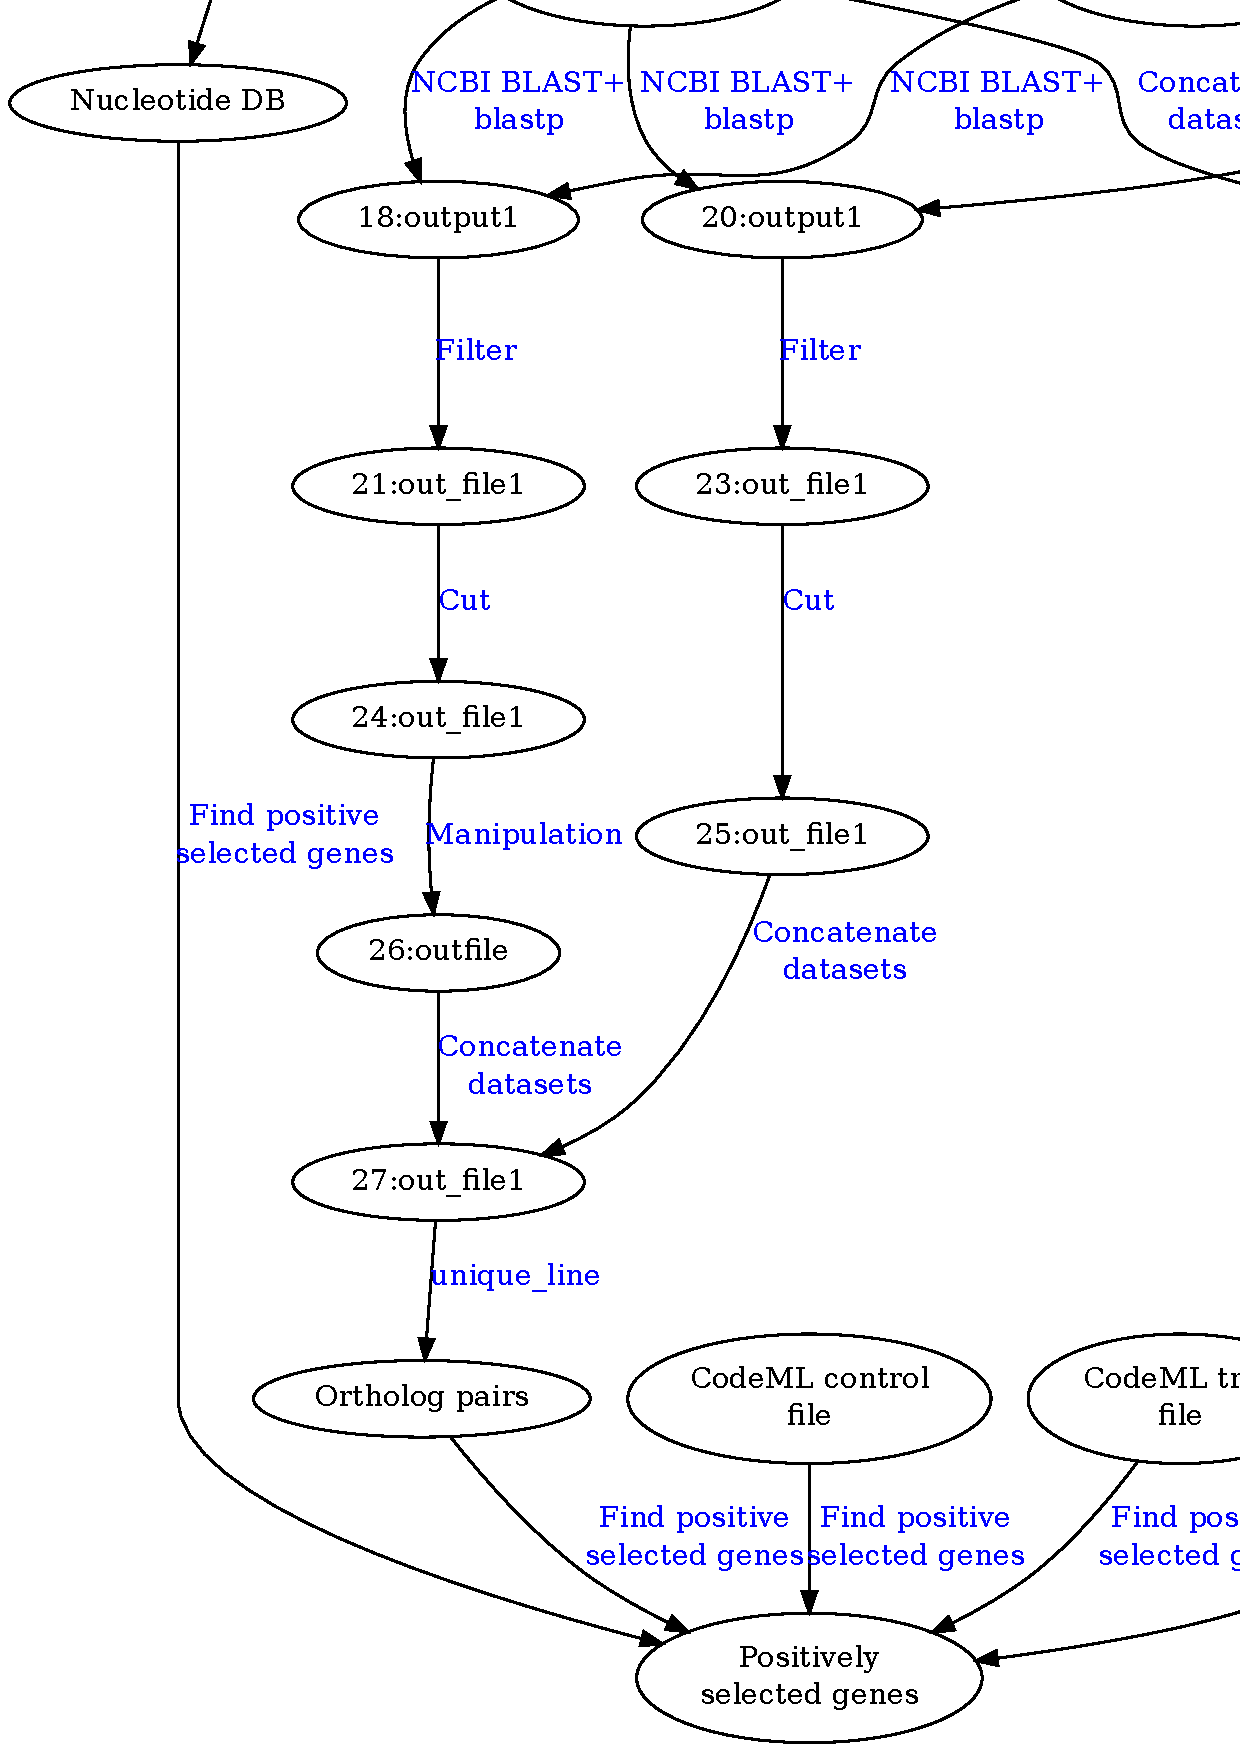
\includegraphics[width=0.7\textwidth]{images/GalaxyPositiveSelectionPipeline.png}
\caption{Positively selected genes workflow in the Galaxy workflow editor}
\label{fig:GalaxyPositiveSelectionPipeline}
\end{figure}

After experimentally enacting parts of the workflow manually (using the ``Analyze Data'' panel of Galaxy) a workflow consisting of thirty steps was composed using the Galaxy workflow editor (in the the ``Workflow'') panel. A portion of the resultant workflow is show in Figure \ref{fig:GalaxyPositiveSelectionPipeline}. As can be seen from that figure, Galaxy workflows resemble flowcharts, however, whereas flowcharts describe the flow of control in a program, the Galaxy workflow describes the flow of data between analyses (this distinction is important, as the expressive power of flowcharts has been strongly criticised, e.g. in \cite{brooks_mythical_1995}, but it is not clear that the limitations of flowcharts also apply to dataflow diagrams). In order to accommodate the entire workflow in a graphical representation, the textual representation of the workflow was converted into a graph that could be processed by \textbf{graphviz}, shown as Figure \ref{fig:positive_selection_workflow_graph}. Every node in this 
graph is a dataset, and every edge is an analysis (in other words a transformer or a filter). A second graph that shows the same workflow but with analyses as nodes, is available in Appendix \ref{sec:positive_selection_workflow_analyses_graph}.

\begin{figure}[!htb]
\centering
\includegraphics[width=0.7\textwidth]{images/positive_selection_workflow_graph.png}
\caption{Positively selected genes workflow}
\label{fig:positive_selection_workflow_graph}
\end{figure}

In the workflow depicted, steps that are labelled A and B, and the ones labelled C and D, are equivalent. In the first case (A and B) a Genbank format file that contains genomic sequence combined with annotated features on that sequence is transformed into two separate datasets: a FASTA format file containing only the genomic sequence and a Generic Feature Format (GFF3) description of the genomic features. This description of features is then filtered to extract only the gene features, and these are used, in combination with the genomic sequences, to generate a collection of gene sequences (labelled ``nucleotide FASTA'' for strain 1 and strain 2). The genomic sequences are translated to amino acids to yield the proteins that correspond with the known genes (datasets labelled ``protein FASTA''). These are then compared against one another, using the BLAST sequence homology search tool to find matching pairs of genes (i.e. orthologous\footnote{In genomics two genes are orthologous if they are share an origin 
in a common ancestor.} genes). The steps labelled A and B are roughly equivalent to Panji's \textbf{ortho\_BLAST.pl} script. Meanwhile the workflow has forked off processes that combine the sets of genomic and protein sequences to generate indexed sequence databases (that will be used at later steps in the analysis).

\begin{figure}[!htp]
\centering
\includegraphics[width=0.7\textwidth]{images/Subworkflow.png}
\caption{Subworkflow for doing Log-Ratio Test on pair of gene sequences}
\label{fig:Subworkflow}
\end{figure}

The BLAST homology search outputs results in tabular format, where each row consists of a pair of matching sequences and associated information. These matches are filtered to find hits with at least 50\% similarity, and a projection is done to extract only the columns containing the sequence identifiers. Finally the results of the two searches are combined and duplicates are removed. This results in a collection of set of orthologous genes, where each gene is identified by a pair of sequence identifiers (known as ``accession numbers''). Having identified orthologous genes, the workflow now needs to test each pair of orthologs to see if the differences between their sequences indicate positively selected mutations. This is done in Panji's workflow using the scripts \textbf{accession\_to\_gene.pl}, \textbf{in\_frame\_codon\_align.pl}, \textbf{codeML.pl} and \textbf{parse\_codeML\_LRT.pl}. Using tools from the EMBOSS \cite{rice_emboss:_2000}, ClustalW \cite{larkin_clustal_2007} and PAML \cite{yang_paml_2007} 
software suites, a Log-Ratio Test is performed to find ortholog pairs that are positively selected (with a 95\% confidence level, using the chi-squared distribution). A workflow analogous to Panji's was constructed in Galaxy (see Figure \ref{fig:Subworkflow}), but here Galaxy's limitations proved fatal: Galaxy does not support the iteration operation, and thus it is not possible to apply a workflow iteratively across a data collection. The sub-workflow was thus re-implemented as a Python script (the item labelled ``Positively selected genes'' in Figure \ref{fig:positive_selection_workflow_graph}) and then added to Galaxy as a tool that could take the outputs of the preceding workflow steps.

While Panji's workflow executes tools in an entirely sequential fashion, the growth in multi-core CPUs and the use of computing clusters (\cite{stein_towards_2008}) means that very often iterative workflows in bioinformatics are executed in parallel, for example by splitting the input dataset into partitions that can be executed independently. Since at least the 1970s it has been recognised that dataflow specifications enable parallelism \cite{gostelow_view_1979}, and Galaxy supports this pattern of task parallelism in the tool definition language (using the undocumented <parallelism> tag), and this capability was used to add support for parallel execution to the sub-workflow, splitting the input dataset into eight parts that could be analysed in parallel. Since parallelism is specified in the definition of a tool, and since the tool definition is de facto static, Galaxy's support for parallel execution is neither responsive to the size of the dataset (an eight way split might, for example, not make sense 
for a dataset of ten items) nor to resource constraints in the execution environment (in a shared compute cluster, the degree of parallel execution needs to be balanced by the need to share computing resources between many users).

Finally, it is worth noting that Galaxy executes each task independently. When tasks are executed locally, this might not be much of a concern, but in many computing environments the process of setting up and tearing down execution units (for example jobs on a compute cluster or grid) involves overhead. Thus in the steps marked C in Figure \ref{fig:positive_selection_workflow_graph}, dataset 18 is first filtered, then the output of that operation (dataset 21) is transformed through a projection that selects a number of columns (yielding dataset 24) and finally a further text manipulation is performed to yield dataset 26. Such a sequential sub-workflow could be transformed (via ``edge contraction'', i.e. the combination of analyses steps that operate on a chain of datasets) into a single analysis that could be executed as a single unit.

In conclusion, Panji's workflow could be implemented in Galaxy, and fairly rapidly. Doing so involved adding tools to Galaxy, some of which were available via the Galaxy Toolshed and thus could be installed without leaving the Galaxy web-based user interface (although doing the installation required administrative privileges that typically would not be available to ordinary users), but three tools had to be added by writing Galaxy tool descriptors in XML, and editing Galaxy's configuration files. The shift in idiom between the Galaxy web-based environment and the command line environment required to add tools to Galaxy is quite significant. In addition, one of the tools added was an implementation of a sub-workflow, and thus would probably not be reuseable outside the context of the current workflow. Galaxy's lack of support for workflow iteration and sub-workflows forced this form of implementation. In addition, while parallel iteration of sub-workflows is somewhat supported by the (as yet undocumented) 
parallelism tag in the tool descriptor XML, the degree of parallelism can not be chosen at runtime. Finally, executing each step of the workflow as its own task leads to inefficiencies that might be avoidable with a less naive workflow execution engine.




%As can be seen from the diagram, the workflow involves an unconditional fork, where data is prepared in %parallel, before the list of orthologous genes produced by \textbf{reciprocal\_gene\_ID.pl} is created. %This list of genes is then iterated across, with each pair of orthologous (i.e. related) genes being %examined individually, with the results of their analysis finally being presented as a spreadsheet.

%Input data: Genbank / NCBI not supported
%Edited clustalw xml
%phylip format - 10 char limit
%emboss tools - millions of options
%syntax flow vs semantics
  
\subsection{Case study 2: Mapping methylated regions in a bacterial genome}

Deoxyribonucleic acid (DNA) is the molecule that contains the genetic instructions in the cells of every living thing. This molecule is made out of repeating sub-units called ``bases''. In general there are four types of DNA base, adenine, thymine, guanine and cytosine. The combination of these bases describes the sequence of amino acids that make up proteins. The process of creating a protein sequence from a DNA sequence involves a sub-process called transcription. Transcription in cells is regulated, thereby ``switching'' genes on and off, and altering the production of proteins. One mechanism involved in transcription regulation is methylation, where a methyl group is added to the cytosine base. Detecting methylation in a genome is important for understanding gene regulation and thus the molecular biology of an organisation. Alecia Naidu, a doctoral student at SANBI is studying this process in bacteria and they have implemented their analysis workflow in Galaxy. They were approached to document their 
workflow via a series of interviews.

In order to detect methylation, DNA is treated with bisulfite. This converts unmethylated cytosine basis to uracil, but methylated cytosine bases are unchanged. Thus, methylated bases can be detected by comparing the sequence of bases in bisulfite treated DNA with that of untreated DNA from the sample biological sample. An image of the workflow that Naidu produced is included as Figure \ref{fig:canvasworkflow_blurred}. The details of most of the analysis steps are blurred out since this work is, as yet, unpublished. In general, however, the workflow involves transforming a set of input nucleotide reads from the sequencing of a bisulfite treated genome into a set of predicted methylation sites by combining the read dataset with a reference genome dataset. In other words, it complies with the transform and filter task schema that Stevens et al outlined. The author has had some experience with producing workflows using the command line and scripting languages, and their assessment of Galaxy is not positive. 
They compared the process of doing bioinformatics in Galaxy to "doing bioinformatics using blinkers", and in particular noted the fact that the tool wrappers of Galaxy do not always expose the full set of command line switches that some tools support. This is an understandable omission given the vast number of options available for some tools (for example, the \textbf{tranalign} tool from the EMBOSS tool suite has 51 different command line switches).

\begin{figure}[hbt]
\centering
\includegraphics[width=\textwidth]{images/canvasworkflow_blurred}
\caption{Methylation analysis workflow (details blurred out)}
\label{fig:canvasworkflow_blurred}
\end{figure}

In addition, Naidu noted that each dataset is different, and that this made the details of the workflow to some extent dependent on the characteristics of the input data. For example, the accession number that is used to identify a nucleotide or amino acid sequence might sometimes also contain further information in its formatting, thus a tool might need to act differently depending on the formatting of this sequence identifier. This kind of complexity requires that the workflow user has detailed knowledge of the bioinformatics applications used in the workflow and thereby the ability to hide complicity using the workflow abstraction is reduced.

In addition, the Galaxy workflow abstraction does not allow the user to specify the resource requirements of analysis steps. In a cluster or grid environment this is typically something that is specified at job submission time, and might be used to allocate particular tasks to different nodes in a computing environment. This was a concern to Naidu because the analysis that their are enacting is resource intensive, requiring a computer with more than 15 GB of RAM in order to process. In addition to being resource intensive during processing, Naidu's analysis involves considerable grow in data storage requirements. Their test dataset is 360 MB in size and by the end of the analysis some 2.6 GB of disk space is used by all the datasets involved in the workflow. In Figure \ref{fig:canvasworkflow_blurred}, the FASTQ Groomer steps simply transforms an input dataset from one input format to another for use in later analysis, yet the duplicate dataset is retained. The next step, the FASTQ trimmer, transforms its 
input by performing ``quality trimming'', but once again the input dataset is retained in its entirety.

Finally, Galaxy does not support the suspension and resumption of workflows, thus a failure in any one of the workflow's steps would require re-executing the workflow in its entirety. This is different from the experience of command line bioinformatics workflows where analysis steps can be manually re-enacted as needed. Thus, while Naidu's workflow is a fairly straightforward transform and filter operation, they have experienced considerable frustration in implementing it in Galaxy and thus complain that the Galaxy environment ``doesn't do what it promises''.

\subsection{Case study 3: Exploring the impact of k-mer length on assembly quality}

In the first decade of the 21st century DNA sequencing has been revolutionised by a set of technologies that are collectively known as ``next generation sequencing'' (NGS)\cite{shendure_next-generation_2008}. Instead of producing runs of tens or hundreds of thousands of sequence fragments, these technologies produce millions of sequence fragments (known as ``reads'') in a single day. These individual sequence reads (each of which is typically between 50 and 500 bases long) need to be combined to recover the complete sequence that has been sequenced. This process is known as assembly, and for NGS techniques based on the use of de Bruijn graphs are common \cite{compeau_how_2011}. DNA assembly results in fragments of contiguous of sequence, called contigs. The length of these contigs can be used to judge the quality of an assembly, and in general, an assembly that has longer contigs is a better assembly. A statistical measure, $N50$, is used to rate contig length, and thus assembly quality \cite{burton_n50_2008}
\footnote{The $N50$ measure describes the length $N$ for which 50\% of the bases in the assembly are in contigs shorter than $N$}.

Stanley Mbandi-Kimbung, a doctoral student at SANBI, was approached to describe their workflow for assessing the quality of assemblies produced by the \textbf{velvet} \cite{zerbino_velvet:_2008} and \textbf{oases} \cite{schulz_oases:_2012} tools. The first of these, \textbf{velvet}, is an assembler that uses a de Bruijn graph based approach to compute the correct assembly of a set of genome fragments and one of the key parameters used by \textbf{velvet} is the length of the DNA fragment used as a ``word'' during the de Bruijn graph construction. This is the ``k-mer length'', and Mbandi's pipeline varies this parameter while keeping all other input to the assembly process constant. This workflow is thus an example of a ``parameter sweep'', where a parameter space for a tool is explored to try and discover the optimal parameter set. Mbandi implemented this workflow in the form of a Perl script (available in Appendix \ref{sec:velvet_assembly_parameter_walk})\footnote{Recent versions of \textbf{velvet} include a 
script named \textbf{VelvetOptimiser.pl} that implements a similar workflow.} that operates according to the logic show in \ref{fig:oases_parameter_walk}. For simplicity's sake the \textbf{oases} step has been left out since that does nothing besides post-processing the assembly produced by velvet.

\begin{figure}[!htb]
\centering
\includegraphics[width=0.5\textwidth]{images/oases_parameter_walk}
\caption{Mbandi's parameter sweep of the velvet assembler}
\label{fig:oases_parameter_walk}
\end{figure}

The workflow takes as input a set of sequence reads from a DNA sequencing experiment (in practice Mbandi used a set of about 10 million reads from the fungus \emph{Venturia inequalis}) and a parameter range describing a set of k-mer lengths. For each k-mer length, the \textbf{velveth} program is run to build up information on which k-mers exist and in which sequences they are found. Then the \textbf{velvetg} program is run to assemble the reads using a de Bruijn graph, and produce (amongst others) a file containing assembled contigs. Finally the contig file is analysed to produce a $N50$ value and the $N50$ value and its associated k-mer parameter are stored.

\begin{figure}[!htb]
\centering
\includegraphics[width=0.5\textwidth]{images/ComputeVelvetAlignments}
\caption{Velvet parameter sweep implemented in parallel}
\label{fig:ComputeVelvetAlignments}
\end{figure}

While Mbandi's workflow iterates through the parameter set, the workflow conforms with the van der Aalst et al's ``multiple instances with a priori knowledge'' workflow pattern, since each the number of sub-workflows is known at the outside, and one could execute the \textbf{velvet} tool for each k-mer value in parallel, resulting in the workflow as showing in Figure \ref{fig:ComputeVelvetAlignments}. An analysis of Mbandi's workflow in terms of data flow instead of control flow naturally elicits this parallelism. While enacting the workflow resource constraints should be borne in mind (as in Naidu's workflow discussed above) since even on Mbandi's relatively small set of reads the \textbf{velvet} tool uses approximately 1.5 GB of RAM during its execution.


An attempt was made to implement this workflow in Galaxy, and in the process it was discovered that the \textbf{VelvetOptimiser.pl} tool (and the corresponding tool for \textbf{oases}) has been incorporated into a tool available in the Galaxy Toolshed. Galaxy itself is, however, unsuitable for implementing a parameter sweep because when a workflow is composed in Galaxy the parameters used are fixed at Workflow composition time, and at execution time only the dataset can be varied. In addition, as mentioned before, sub-workflows are not supported and these, together with that Castro et al call ``recursion'' are necessary for implementing a parameter sweep. Thus to implement a workflow such a Mbandi's in Galaxy would instead mean to implement the workflow in its entirety outside of Galaxy and simply invoke the resulting implementation as a single tool.



%\subsection{Themes}
%
%\begin{itemize}
%
% \item Galaxy in context: evaluate Galaxy according to the schema proposed in \cite{deelman_workflows_2009}
%
% \item Workflow patterns: what workflow patterns (following \cite{van_der_aalst_workflow_2003} are used in bioinformatics workflows. What patterns are supported in  Galaxy.
%
% \item Workflow evolution: what is involved in extending Galaxy in order to accomodate analyses that are not supported ``out of the box''. To what extend is this extension / evolution supported or is there an ``impedence mismatch'' between the terminology / conceptual world of workflows and the terminology / conceptual world of workflow instantiation / execution.
%
% \item Resource allocation: How does Galaxy interact with concerns for efficient usage of available resources? (linked to above theme, ability to address resource allocation well) How has this been addressed in other workflow systems?
%
% \item Support for abstraction: In order to be re-useable, programming constructs, including workflows, require support for a certain amount of abstraction. In real world examples, what aspects of workflows do researchers expect to be parameterised, and thus what forms of abstraction are required. To what extent are these available in Galaxy (and other scientific workflow systems).
%
%\end{itemize}

\section{The features of Galaxy as a workflow system}

In the introduction to this research report I cited the suggestion that \gls{BSA} faces an ``informatics crisis'' characterised by the accumulation of data without a concomitant increase in analytical capacity. This ``informatics crisis'' is not a phenomenon unique to bioinformatics and as a result scientific workflow systems have been widely used outside of the field. Yu et al mention their use in fields as varied as astronomy, geophysics and bioinformatics. \cite{yu_taxonomy_2005} The case studies detailed above, together with Stevens and Castro's more theoretical overview, shows the elements involved in the challenge of bioinformatics. Approaching the question of Galaxy's ability to contribute as a tool for enacting bioinformatics workflows, I will now consider the capabilities of scientific workflow systems in a more general sense. Both Deelman et al \cite{deelman_workflows_2009} and Yu et al \cite{yu_taxonomy_2005} have proposed classifications of workflow features, and I will now illustrate how these 
features relate to both the concrete bioinformatics workflows and the feature set exhibited by Galaxy. Deelman et al suggest that workflow systems should be be classified according to their support for:

\begin{enumerate}
\item Workflow composition
\item Mapping workflow specifications to executable resources
\item Workflow execution
\item Support for recording data provenance
\item Interoperability with other workflow systems
\end{enumerate}


\subsection{Workflow composition}

Workflows in Galaxy are composed using a graphical tool in what is essentially a graphical dataflow language. Tools are selected from the sidebar, parameters are configured and input and output datasets are represented as ports that can be chained to other tools. Each dataset has an associated format and this information is used to decide which ports can be connected together. The data format is also used when deciding how to display the data in the ``Analyze Data'' pane. Each dataset also has associated metadata that describes it, for example the genome it is associated with. In terms of the workflow structures that Yu et al \cite{yu_taxonomy_2005} consider, Galaxy workflows are Directed Acyclic Graphs (DAGs) that support parallelism (the output of a single tool can be input to more than one downstream tool) but not choice between dataflow paths.

Deelman et al \cite{deelman_workflows_2009} suggests that abstraction is necessary to manage the complexity of graphical representations of workflows. This point is reinforced by Blackwell et al in their survey of the cognitive features of visual programming languages \cite{blackwell_cognitive_2001}, where they speak of an ``abstraction gradient''. What levels of abstraction are possible? The Galaxy workflow composer presents two levels of abstraction: the view of the entire workflow, and the detailed view of the parameters of a single tool. As the case studies have shown, there are a number of common tasks is bioinformatics workflows that Galaxy does not support, and in some cases (such as the duplicated sections of the workflow illustrated in Figure \ref{fig:positive_selection_workflow_graph}) this leads to increased complexity.

Deelman et al and Altintas et al \cite{altintas_framework_2005} makes three suggestions for abstraction in workflows: nesting workflows (i.e. the ability to call sub-workflows), the ability to hide ``shim services'', and abstracting patterns in workflows into ``abstract actors''. The ability to call sub-workflows is the most straightforward requirement that Galaxy lacks. Workflow patterns such as iteration using multiple instances, and parameter sweeps both require sub-workflows to be implemented, as is illustrated by the obstacles encountered in implementing case studies one and three in Galaxy.

Shim services (or tasks) are workflow elements that simply reformat data (in other words they make changes that are simply syntactic). The manipulations that happen to datasets 13 and 12 in the positively selected genes workflow from case study one (Figure \ref{fig:positive_selection_workflow_graph}) are examples of shims. These simply trim off an extraneous piece of text that is added to the sequence identifier by transeq. Similarly the FASTQ groomer used in Naidu's workflow (Figure \ref{fig:canvasworkflow_blurred}) simply transforms a FASTQ format file between two different variants of the same sequence format. Galaxy allows the workflow designer to hide the outputs of workflow tasks. This facilites hiding shim tasks and reduces the complexity of the set of datasets presented to the user when a workflow completes. aAt the workflow composition stage it might, however, be useful to be able to hide these shims in order to reduce graphical complexity. This is somewhat related to encapsulating with sub-
workflows, in the sense that a tool and a format altering shim might be conceptually combined into a sub-workflow that appears as a single item in the final workflow.

Finally, Altintas et al suggest that concrete tasks in workflows can sometimes be replaced by abstract actors. This corresponds to the abstract pole on Yu et al's workflow model axis. While Galaxy abstracts away the details of how tasks are executed (thus the same workflow could execute on a single computer and also on a compute grid), the notion that a task itself could be a ``place holder'' is a useful abstraction. Thus, for example, the framework for a parameter sweep evaluation of an assembly tool could be retained and reused with different concrete assembly tools. As workflows are shared and reused this kind of abstraction could reduce the proliferation of workflows that are essentially similar and only differ in a single detail.

The abstractions listed above allow for workflows to be considered from a higher level of abstraction. Another dimension of workflow composition involves the details of the tasks that workflows are composed out of. Currently in Galaxy adding or modifying a tool requires leaving the Galaxy environment and editing XML format text files, or alternately adding the tool from the Galaxy tool shed. There is no way to edit the definition of a tool from within the Galaxy web interface. The NAIAD HPC Web workflow system \cite{tartakovsky_cyber_2011} (itself built upon the Mobyle \cite{neron_mobyle:_2009} workflow system) solves this problem by providing a web form based tool builder. The Galaxy tool definition language (partially documented in \cite{the_galaxy_team_galaxy_2011}) is, however, more complex than the one used in HPC Web, thus it might not be straightforward to implement an equivalent tool builder.

Blackwell et al have suggested that the availability of a well-stocked library of reuseable components elevates the semantic level of a visual programming language. This is certainly true for Galaxy, as the base system comes with more than 300 tools already available, and the Galaxy tool shed provides access to almost 2000 more. A large number of powerful operations are immediately available for inclusion into Galaxy workflows. These tools are complemented with nearly 200 data format definitions. In a sense Galaxy comes ``batteries included'': immediately after installation it is possible to use it for real world work.

Deelman et al suggest that handling of parameters should be considered when surveying workflow system features. The Galaxy workflow system treats datasets as input and output parameters, but they are the only parameters supported in workflow composition. The blocks that represent tools used in workflows have no ports for settings parameters (such as k-mer length for sequence assembly), something that prevents certain kinds of workflows (for example parameter sweeps) from being implemented. The abstract actor proposal that Altintas et al suggest would require a further extension of the Galaxy system, so that tools themselves can be passed as parameters to workflows.

Finally data flow in Galaxy is structured by matching syntax of outputs and inputs. Stein \cite{stein_towards_2008} has suggested that semantic information could be used to guide the construction of workflows. Yu et al and Deelman et al also take up this theme, suggesting that workflow construction might even be partially or fully automated. (An early example of research in this area was the TAMBIS system \cite{stevens_tambis:_2000} and the topic is also explored in Gil et al \cite{gil_artificial_2004}). While the full semantic description of tools is too much to ask for at this point, Galaxy does make use of some semantic information such as the fact that certain data types describe genomic intervals. The new parallelism tool configuration also makes use of the fact that certain data formats in fact describe collections that can be analysed in parallel.

\subsection{Mapping workflows to resources}

Mapping involves translating the abstract workflow description composed by the user into a concrete execution plan. In this regard Deelman et al differentiate between task-based and service-based workflows. In service-based workflows, mapping involves binding to services (often, as in the case of Taverna \cite{hull_taverna:_2006}, web services), where services might be chosen based on suitability and quality of service issues. On the other hand, task-based workflow systems map workflow steps to particular executable resources. Clearly Galaxy is a task-based workflow, and implements mapping through ``job runners''. Executable resources in Galaxy are referred to as tools and the system maintains a registry of tool definitions that, in turn, are specified in a XML based tool description language. The tool registry is loaded at Galaxy startup, and to add new items the Galaxy application needs to be restarted (although, once loaded, the tool definition for individual tools can be updated without restarting the 
entire Galaxy application). Job runners translate a request to invoke a particular tool into the concrete steps required to execute that tool. Galaxy supports local execution (on the same machine as the Galaxy application is running) and execution via a number of batch-queueing systems. The Galaxy administrator can configure the association between individual tools and job runners as well as a default job runner for the Galaxy installation.

Galaxy jobs are scheduled in a centralised fashion, with the scheduler communicating with job runners through a job queue. The Galaxy web interface translates user actions into job specifications that are placed on the queue queue, and job runners (each with a configurable number of threads of execution) consume jobs from the job queue and manage the execution of the tools specified in the jobs. In the case where Galaxy interfaces with a batch-queue system the limitations of the Galaxy mapping system becomes apparent, since while modern batch-queueing systems possess sophisticated schedulers that can route jobs to appropriate computing resources based on characteristics such as user role, expected memory utilisation or execution duration, Galaxy provides no such information to the batch-queueing system. Instead, all jobs are scheduled by a single system user with no resource information supplied. Other workflow systems, such as Triana \cite{churches_programming_2006}, allow workflow specifications to be 
annotated with information that can be used in scheduling decisions, such as which elements are compute intensive. Another approach, used by the ICENI workflow system \cite{mcgough_workflow_2004}, is to use some form of metric to try and estimate resource usage based on input data characteristics.

Finally, workflow mapping offers the possibility of workflow optimisation. Deelman et al mentions sophisticating optimisation of task-based workflows carried up by Pegasus \cite{deelman_pegasus:_2005} and Askalon \cite{fahringer_askalon:_2005}. These involve analysing the DAG that describes a workflow and applying operations such as task clustering. Galaxy does not perform any such optimisations, with the result that even shim tasks are scheduled independently of the analyses they bind together. Since Galaxy generates an internal DAG representation of the workflow, adding an optimiser to the system should be quite feasible and this would have significant performance advantages.

\subsection{Workflow execution}

Once a workflow has been translated into a concrete specification of tasks to be executed, the actual execution of tasks needs to be managed. Galaxy manages this through the communication between the Galaxy scheduler and the job runners. Task execution involves not just running tools, but also the operation that surround the execution of a tool. For example data might need to be transferred to the location of execution (stageing in) and results downloaded after execution (staging out), authentication might need to be managed (for example, in order to access resources on a compute grid) and the tool might require particular environment variable to be set. While some Galaxy job runners do support stageing in and stageing out, in general Galaxy assumes that both the Galaxy application server and the tools it executes will have access to a shared filesystem space (typically shared using NFS). Galaxy users authenticate to the Galaxy web application, and there is experimental support for mapping users on the 
Galaxy web app to users on the system that Galaxy is executing on. There is clearly much scope for improvement in how Galaxy manages tool execution, as the management of the complexities involved in this domain seems somewhat ad-hoc at present.

In addition to the details of how to execute a task, a workflow system is often faced with the failure of a particular task execution. This failure might be permanent, for example in the case where a tool is incorrectly implemented, or transient, for example where a resource such as disk space is temporarily exhausted. As workflows increase in complexity, failure of an component becomes increasingly likely, and in their study of fault tolerance in scientific workflows, Kandaswamy et al \cite{kandaswamy_fault_2008} found that of 165 weather forecasting workflows run on the US TeraGrid in one month, 131 encountered a task failure. Utilising a fault recovery service, 93 of these failed workflows were successfully recovered, reducing a workflow failure rate from 79\% to 23\%. Bowers et al propose certain patterns of fault recovery (in other words exception handling) that can be applied to the Kepler workflow system \cite{bowers_enabling_2006}. At present Galaxy does not have any fault tolerance features, and the 
failure of a single task leads to the abort of the entire workflow downstream from that task. Tasks that do not depend on the failed task continue to run, thus a workflow might exhibit partial success. The concern with fault tolerance lies in a space that where workflow execution and workflow mapping overlap to some extent, since one response to failure (for example of a compute node) might be to reconsider the mapping between an abstract workflow and its concrete execution plan. Yu et al refer to this capability as dynamic planning, and as Bowers et al's work shows, it is an area where concern with the flow of control appears even if the workflow is specified in terms of data flow.

One aspect of control flow is that is related to fault tolerance is pause and restart capability. A user might identify and remedy the cause of a failure, and wish to restart a workflow from a particular step onwards. Deelman et al mention that Askalon supports workflow checkpointing to facilitate such a restart. Galaxy, however, does not support any notion of workflow pausing or restarting. In essence, if control in a workflow can be imagined as a set of tokens that passes from task to task, Galaxy does not support any mechanism for the user to manipulate such control tokens. The result is that workflow execution in Galaxy can be a frustrating fragile process.

\subsection{Support for recording data provenance}

Data provenance is a record of the history of the creation of a data object. In ``traditional'' bioinformatics workflows, like Panji's positive gene selection workflow, datasets are produced without any information being captured about how they are produced, except for the documentation produced by workflow authors. Goecks et al point out the weakness of this approach, citing a study showing that less than half of a particular set of microarray experiments could be reproduced, with missing data and data provenance information being a large factor in the inability to reproduce experimental result. Galaxy addresses this problem by recording provenance information about datasets with each item produced. Information about inputs, outputs, tools used, tool XML version and tool parameters is stored, and can be shared between users on a Galaxy instance or exported as a file. The Galaxy system can also be used as a kind of content management system for scientific publications, where Galaxy tools, workflows and data 
library items can be embedded in a web page. As far as I know, Galaxy is the only platform that allows for this kind of publication.

Apart from data provenance, Deelman et al note that it is useful to track the history of changes to a workflow and that transformation of a workflow (for instance by workflow optimising by the scheduler) could impact on the provenance information recorded. Galaxy does not support workflow versioning, nor does it transform workflows in any significant way, except for optionally hiding datasets in the user's history. Besides ensuring reproducible research, stored data provenance information could be used to reduce the disk space usage of a workflow. As another example, a workflow implemented at SANBI for the analysis of novel tuberculosis strains generates some 60 GB of data for each strain of the bacteria analysed. Only a small fraction of this is input data and analysis results, the bulk is intermediate datasets used within the workflow. With sequencing now under way for hundreds and maybe even thousands of strains of Mycobacterium tuberculosis, the ability to identify which datasets may safely be erased (
and possibly recomputed at a later date if necessary) could save terabytes of disk space. At present, however, Galaxy does not itself erase any data, not even datasets marked ``deleted'' in the user's history. Site administrators are advised by the Galaxy developers\footnote{See \href{http://wiki.g2.bx.psu.edu/Admin/Config/Performance/Purge\%20Histories\%20and\%20Datasets}{Purge Histories and Datasets} in the Galaxy documentation.} to clean up their disk space by periodically running a ``clean up'' script that examines the Galaxy database and deletes datasets that are marked as deleted. If data provenance information were extended to include information about the resource cost of computing a dataset and about which datasets needed to be retained as analysis results, the Galaxy provenance data system could be a powerful tool for disk usage management.

\subsection{Workflow interoperability}

A bioinformaticist searching for a workflow system is faced with a dizzying array of choices. Searching 
the web for bioinformatics workflow systems reveals Galaxy \cite{giardine_galaxy:_2005}, Taverna \cite{oinn_taverna:_2004}, Kepler \cite{altintas_kepler:_2004}, Triana \cite{churches_programming_2006}, Bioopera \cite{bausch_bioopera:_2002}, Mobyle \cite{neron_mobyle:_2009}, BiosFlow \cite{xu_biosflow_2009}, \cite{orvis_ergatis:_2010} and bpipe \cite{sadedin_bpipe:_2012}, amongst others. Each of these workflow systems uses a different format for storing and exporing its workflow descriptions and there are often semantic differences between the systems, for example Taverna's service-based structure compared to Galaxy's task-based one. It is unrealistic (at this stage, at least) to expect workflow system designers to decide on a single language for specifying scientific workflows, but some work has been done on making Galaxy interoperate with other workflow systems. 
In particular, Wang et al \cite{wang_adapting_2009} and Abouelhoda et al \cite{abouelhoda_meta-workflows:_2010} have attempted integration between Galaxy and web services based workflow systems.\footnote{In the terminology of the Workflow Management Coalition, both forms of integration involve cooperation between different workflow systems, i.e. Level 2 interoperation \cite{workflow_management_coalition_workflow_1999}.} Wang et al implement this by creating a tool that converts Web Service Definition Language (WSDL) descriptions into Galaxy tool and datatype specifications. Similarly, Galaxy exposes a XML-RPC based API that allows workflows in Galaxy to be called by external programs. This API is still, however, experimental and undocumented (except through code examples).

Abouelhoda's approach is on a higher level of abstraction, in that they present an abstract workflow specification that is converted into sub-workflows that are executed either by Galaxy or Taverna\footnote{The result is a tool dubbed \href{http://www.tavaxy.org/}{Tavaxy}.}. The choice of which workflow system to execute sub-workflows on is made based on the workflow pattern exhibited by the sub-workflow. This form of integration grasp that workflow interoperability is not simply a matter of building interfaces between workflow systems, since interoperability needs to recognise the semantic differences between workflow systems. For example, a workflow system that is service-based requires different mapping logic (as a choice needs to be made between different instances of the same service specification) to a task-based one.

\section{Conclusion}

Bioinformatics is currently characterised by a disconnect between the vast growth in repositories of biological data and the very slow growth in the capacity to analyse this data. The main constraint on the growth of analytical capacity is a human constraint: the prevalent paradigm of bioinformatics workflow construction requires programming skills on the part of the analyst and these skills are not widely available. In addition, the majority of bioinformaticists come from a life sciences background where training in programming is not common, thus the field is constantly accepting scientists who are not experts at orchestrating computation. This situation has been described as an ``informatics crisis'' \cite{goecks_galaxy:_2010} and has spurred the search for tools that allow scientists to ``[ask] complex questions of the genome without programming'' \cite{woollard_asking_2010}.

One early approach to making bioinformatics tools more accessible to non programmers was to provide web interfaces for what would otherwise be command line tools. Any number of ad-hoc web wrappers exist for individual tools, but projects such as Pise \cite{gilbert_pise:_2002} and wEMBOSS \cite{sarachu_wemboss:_2005} extended this approach by providing a way to automatically generate web based user interfaces from tool descriptions. Such tool interfaces were combined with authentication and dataset management functions to provide web portals for bioinformatics. In its earliest incarnation Galaxy \cite{nekrutenko_introduction_2011} was an example of such a portal, combining interfaces to analysis tools with the ability to import data from biological databases such as the UCSC Genome Browser. From the start Galaxy emphasised storing data provenance information in users' histories and this feature even gave its name to the Galaxy user interface (the History User Interface \cite{giardine_galaxy:_2005}). More 
recent incarnations of Galaxy retain these features and the system is a powerful portal for providing web based user interfaces to bioinformatics tools, executing these tools and visualising results. As a bioinformatics portal Galaxy is powerful, with the Galaxy baseline system providing interfaces to some 300 tools, and the Galaxy tool shed allowing the installation of almost 2000 additional tool interfaces.

The user history metaphor used in Galaxy lends itself naturally to the notion of workflows, where a workflow describes the chaining of a number of different analysis tasks to build a more complex overall analysis. Stevens et al \cite{stevens_classification_2001} and Castro et al \cite{castro_workflows_2005} have categorised the tasks involved in bioinformatics and their classification suggests that workflows are a natural metaphor for answering complex problems bioinformatics. These classifications in turn seem to be expressed naturally in the form of visual dataflow languages. Dataflow computing describes computational tasks in terms of the flow of data between instances of computation \cite{gostelow_view_1979} as opposed to the more common paradigm in programming that describes the flow of control in a program.

Dataflow computing provides an explicit description of the combination of data and tools that needs to be present at the moment of computation. As Gostelow \cite{gostelow_view_1979} showed as long ago as 1979, dataflow description lends itself quite naturally to composing parallel execution plans that can be mapped to resources on the many-core compute clusters, grids and clouds available to scientists. Visual dataflow languages also have a long history, with Hils \cite{hils_visual_1992} providing an early overview and Blackwell et al \cite{blackwell_cognitive_2001} discussing cognitive factors that affect their expressive power.

Thus, to recap, workflow systems that allow the user to compose workflows in the form of visual dataflow descriptions provide a powerful tool to ask complex questions about biological data without resorting to programming. Galaxy is one amongst a number of workflow systems that allow users to compose workflows in this manner. The workflow composition and enactment components of Galaxy are, however, limited in ways that make doing real-world bioinformatics in the system challenging.

Firstly, in terms of workflow composition, the Galaxy workflow system does not allow for a smooth ``abstraction gradient'' that would allow users to switch between high level overview of workflow tasks and drilling down into the details of workflow task definition. Tool definition in Galaxy happens outside of the web user interface, thus one is forced to be familiar with the XML tool declaration language in order to extend the set of tools that Galaxy supports. On the other side of the scale sub-workflows are not supported so workflows can not be encapsulated and reused within other workflows.

Castro et al \cite{castro_workflows_2005} specifies two operations in bioinformatics that operate across collections. On the one hand what they call iteration operates across a collection of data items, applying the same operation to each one. On the other hand what they call recursion operates across a set of input parameters, executing a parameter sweep where the these parameters are used to alter an operation that is repeatedly executed on the same dataset. Both of these constructs require the support in a workflow system for bioinformatics, and neither is supported. Deelman et al \cite{deelman_workflows_2009} suggests that such constructs can be well supported by combining control flow and dataflow descriptions in workflow composition. Bowers et al \cite{bowers_enabling_2006} concur with Deelman et al and provide a model of where a workflow can consist of dataflow description on a high level but incorporate control flow elements in a lower level description of workflow tasks. 
Elizondo et al \cite{velasco_elizondo_catalogue_2010} propose that instead of providing this description on the task level, the necessary constructs can be expressed using a suitable library of component connectors. Whichever route is chosen, to make Galaxy useful for general purpose use, one of these solutions needs to be adopted. In addition, Altintas et al \cite{altintas_framework_2005} propose a further level of abstraction: tasks in a workflow might be place holders, allowing the same abstract workflow description to be reused with the place holder replaced at run-time with one or another concrete analysis task. For example, a general workflow for mapping novel sequence reads to a genome can be produced, and the choice of which mapping tool to use can be left for a moment close to run-time.

Moving along the abstraction gradient could also allow semantically uninteresting elements of a workflow, such as data format conversion shims, to be hidden in a high level workflow description. In addition to this navigation of several levels of abstraction, the Galaxy workflow system needs to be extended in terms of how the system maps workflow descriptions to execution plans. At the moment Galaxy does this in a naive manner, simply queuing up jobs for job runners to execute. There is no scope for expressing resource requirements such as the amount of memory or the duration of runtime that a task might require. Enhancing Galaxy workflow description with a way of expressing resource requirements would allow more detailed execution plans to be prepared. In addition, since Galaxy is aware of the workflow description in its entirety prior to workflow execution, the Galaxy scheduler could be enhanced to optimise execution steps, grouping steps together that share datasets, for example.

Once the Galaxy scheduler has transformed a workflow description into an execution plan, execution is effected through job runners that provide an interface to various batch-queue systems, as well as allowing tools to be executed directly on the local system. While Galaxy does an impressive job in abstracting away the differences in how analyses are executed, and thereby hiding the tricky details of computation from its users, the complexities of tool execution, in particular the stageing in and out of data and managing user authentication to computational resources is handled in a fairly ad-hoc manner. Some of this is no doubt due ot the experimental nature of these features of Galaxy, but in event it is an area that could do with improvement.

Finally, a more significant weakness is Galaxy's lack of support for fault tolerance and recovery. If a task within a Galaxy workflow fails to execute correctly, there is no way to restart part of a workflow. As workflows grow in complexity, the chance for task failure increases, and some form of fault recovery becomes imperative. This might take the form of exception handling, manual retry of failed tasks or a fault recovery service that automatically retries failed components. Manual fault recovery is probably the simplest idea to implement, but this would require making explicit the manipulation of control flow in the workflow, possibly through a way to stop and start particular workflow steps individually. An alternative is to generate a series of checkpoints as the workflow executes and allow the user to re-execute the workflow from a particular checkpoint.

In spite of these weaknesses, Galaxy is widely used for real world bioinformatics, with the public Galaxy server (\url{https://main.g2.bx.psu.edu/}) processing over 130 000 jobs per month and accepting more than one terabyte of data uploads every week. \cite{nekrutenko_introduction_2011} As the examination of the cases studies in my research make clear, however, Galaxy does not yet provide an environment capable of replacing the command line and scripting workflow style in use in bioinformatics. This is unfortunately as some of the features of Galaxy, for example, its handling of data provenance, are a significant advance over the shell script and command line style of bioinformatics. Galaxy's limitations are not, however, fundamental limitations of scientific workflow systems, and a survey of the field of scientific workflow systems suggests that they might provide a powerful tool to address the ``informatics crisis''. Certainly as biological data accumulates there is pressure to both reach the same answers 
faster (thus we cannot afford to spend years on sequence assembly problems anymore) and to ask more complex questions of the data. In the absence of a sudden increase in scientists who are also programmers, tools that allow non programmers to ask questions of biology data are crucial. Galaxy in its incarnation as a web portal and naive workflow composition and execution environment is already one such tool, and the limitations identified in this research clearly don't stop Galaxy being used. Instead they could be seen as presenting an agenda for further research, a set of tasks the bioinformatics programmer community can adopt whose pay off is likely to be substantial.

\printglossary

\cleardoublepage
\phantomsection
\addcontentsline{toc}{chapter}{Bibliography}
\bibliography{Workflows,DataExplosion,BioinformaticsSkillsDevelopment,Bioinformatics,SoftwareEngineering,Dataflow,ShortReadAssembly}

\appendix
\appendixpage
\addappheadtotoc


\chapter{Positive selection workflow}

\label{sec:positive_selection_workflow_analyses_graph}

While Figure \ref{fig:positive_selection_workflow_graph} displays datasets as nodes of the graph, the Galaxy workflow editor uses analyses as nodes of the graph. Thus \ref{fig:positive_selection_workflow_analyses_graph} shows the workflow with analyses as nodes and datasets as edges.

\begin{figure}[h!]
\centering
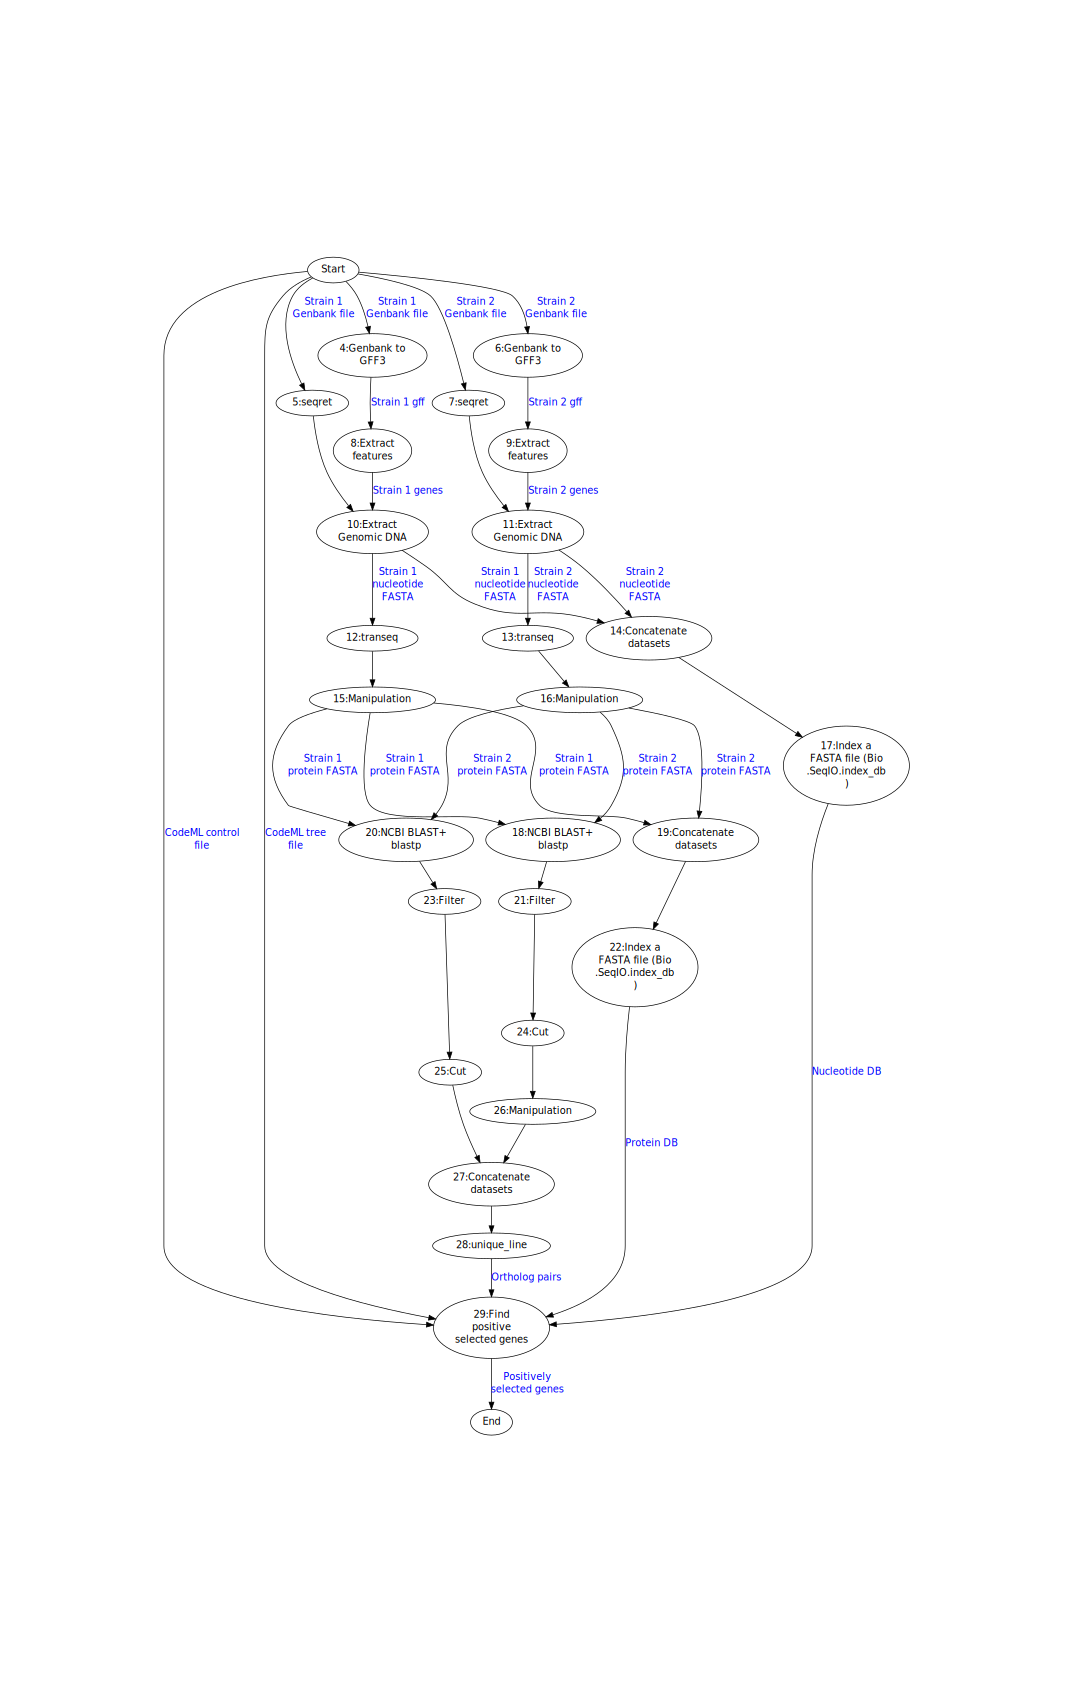
\includegraphics[width=0.9\textwidth]{images/positive_selection_workflow_analyses_graph.png}
\caption{Positively selected genes workflow with analyses as nodes}
\label{fig:positive_selection_workflow_analyses_graph}
\end{figure}

\chapter{Velvet assembly parameter sweep}

\label{sec:velvet_assembly_parameter_walk}

Stanley Mbandi-Kimung's workflow for exploring the \textbf{velvet} and \textbf{oases} parameter space.

\lstinputlisting[language=Perl]{mbandi/symbolic.velveth.ins.pl}

\end{document}